\documentclass[a4paper,11pt]{article}

% ============================================================
%  Le Collé — Séance 1 : Déterminants, courbes paramétrées
%  © 2026 Ahmed Amine Ouqlani
% ============================================================

% ---------- Polices ----------
\usepackage[utf8]{inputenc}
\usepackage[T1]{fontenc}
\usepackage[sc]{mathpazo}          % texte et mathématiques : Palatino
\usepackage[scaled=0.88]{helvet}   % titres et repères : linéale
\linespread{1.07}
\usepackage{amsmath,amssymb,amsthm,mathrsfs,stmaryrd}
\usepackage{microtype}

% ---------- Mise en page ----------
\usepackage[a4paper,top=2.3cm,bottom=2.3cm,left=2.4cm,right=2.4cm,
            headheight=14pt,headsep=0.8cm,footskip=1.1cm]{geometry}
\setlength{\parindent}{0pt}
\setlength{\parskip}{0.45em plus 0.15em minus 0.1em}
\raggedbottom
\emergencystretch=1.5em
\clubpenalty=10000 \widowpenalty=10000 \displaywidowpenalty=10000 \brokenpenalty=10000

% ---------- Couleurs : un bleu de nuit, un ocre, des gris ----------
\usepackage{xcolor}
\definecolor{Ink}{HTML}{1C2533}
\definecolor{Bleu}{HTML}{1F3A5F}
\definecolor{BleuMoyen}{HTML}{4A6A8F}
\definecolor{BleuClair}{HTML}{9DB2C9}
\definecolor{Fond}{HTML}{F2F4F7}
\definecolor{Ocre}{HTML}{B07A26}
\definecolor{Brique}{HTML}{A23B2A}
\definecolor{Gris}{HTML}{5E6672}
\definecolor{Filet}{HTML}{C5CCD6}

% ---------- Packages ----------
\usepackage{enumitem}
\setlist{itemsep=0.25em,topsep=0.35em,parsep=0pt}
\setlist[itemize]{label=\textcolor{BleuMoyen}{\small\textbullet},leftmargin=1.4em}
\setlist[enumerate]{leftmargin=1.8em,label=\textsf{\small\color{Bleu}\arabic*.}}
\usepackage{booktabs,array,multicol}
\usepackage{needspace,float}
\usepackage[font=small,labelfont={sf,color=Bleu},labelsep=period,skip=6pt]{caption}
\usepackage{tikz}
\usetikzlibrary{arrows.meta,calc,decorations.markings}
\usepackage{pgfplots}
\pgfplotsset{compat=1.17}
\usepackage{tkz-tab}
\usepackage[most]{tcolorbox}
\usepackage{titlesec,titletoc}
\usepackage{fancyhdr,lastpage,etoolbox}
\usepackage[colorlinks=true,linkcolor=Bleu,urlcolor=Bleu,citecolor=Bleu,
            pdftitle={Le Collé — Déterminants},pdfauthor={Ahmed Amine Ouqlani}]{hyperref}

\numberwithin{equation}{section}
\numberwithin{figure}{section}
\numberwithin{table}{section}

% ---------- Titres ----------
% numéro du chapitre dans le parcours PT (affiché), distinct de la numérotation interne
\newcommand{\grandnum}{\thesection}\newcommand{\ongletcouleur}{Bleu}
% Chapitres (sections) : grand numéro, titre en linéale, filet ocre
\titleformat{\section}[display]
  {\normalfont\sffamily\color{Ink}}
  {{\small\color{Gris}\textls[200]{\MakeUppercase{Chapitre}}}\\[-0.2em]%
   {\fontsize{64}{64}\selectfont\color{BleuClair}\grandnum}}
  {0.4em}
  {\fontsize{25}{30}\selectfont\bfseries}
  [\vspace{0.5em}{\color{Ocre}\rule{3.2cm}{1.4pt}}]
\titlespacing*{\section}{0pt}{0pt}{1.6em}
\titleformat{name=\section,numberless}[display]
  {\normalfont\sffamily\color{Ink}}{}{0pt}{\fontsize{25}{30}\selectfont\bfseries}
  [\vspace{0.5em}{\color{Ocre}\rule{3.2cm}{1.4pt}}]
\titlespacing*{name=\section,numberless}{0pt}{0pt}{1.6em}

\titleformat{\subsection}
  {\needspace{5\baselineskip}\normalfont\sffamily\Large\bfseries\color{Ink}}
  {\color{Bleu}\thesubsection}{0.8em}{}
\titlespacing*{\subsection}{0pt}{1.8em}{0.5em}
\titleformat{\subsubsection}
  {\needspace{5\baselineskip}\normalfont\sffamily\large\bfseries\color{Ink}}
  {\color{Bleu}\thesubsubsection}{0.7em}{}
\titlespacing*{\subsubsection}{0pt}{1.6em}{0.4em}
\titleformat{\paragraph}[runin]{\normalfont\sffamily\bfseries\color{Ink}}{}{0pt}{}[.]
\titlespacing*{\paragraph}{0pt}{0.9em}{0.6em}
\setcounter{secnumdepth}{3}
\setcounter{tocdepth}{2}

% ---------- Table des matières ----------
\titlecontents{section}[0pt]{\addvspace{0.7em}\sffamily\bfseries\color{Ink}}
  {}{}{\hfill\contentspage}[\addvspace{0.2em}]
\titlecontents{subsection}[2.2em]{\small\linespread{1}\selectfont}
  {\makebox[2.6em][l]{\color{Gris}\thecontentslabel}}{}{\titlerule*[0.7pc]{.}\contentspage}

% ---------- En-têtes et pieds de page ----------
\pagestyle{fancy}
\fancyhf{}
\renewcommand{\sectionmark}[1]{\markboth{#1}{}}
\fancyhead[L]{\footnotesize\sffamily\color{Gris}\leftmark}
\fancyhead[R]{\footnotesize\sffamily\scshape\color{Gris}Le Collé}
\fancyfoot[C]{\small\sffamily\color{Ink}\thepage}
\fancyfoot[L]{\scriptsize\sffamily\hyperlink{toc}{\color{Filet}sommaire}}
\renewcommand{\headrulewidth}{0.4pt}
\renewcommand{\headrule}{{\color{Filet}\hrule height\headrulewidth width\headwidth}}
\renewcommand{\footrulewidth}{0pt}
\fancypagestyle{plain}{\fancyhf{}\fancyfoot[C]{\small\sffamily\color{Ink}\thepage}\renewcommand{\headrulewidth}{0pt}}

% ---------- Énoncés ----------
\newtheoremstyle{enonce}{0pt}{0pt}{}{}{\sffamily\bfseries\color{Bleu}}{.}{0.5em}
  {\thmname{#1}\thmnumber{~#2}\thmnote{\ \normalfont\sffamily\color{Ink}(#3)}}
\newtheoremstyle{exemple}{0.9em}{0.9em}{}{}{\sffamily\bfseries\color{BleuMoyen}}{.}{0.5em}
  {\thmname{#1}\thmnumber{~#2}\thmnote{\ \normalfont\sffamily\color{Ink}(#3)}}
\newtheoremstyle{remarque}{0.7em}{0.7em}{}{}{\sffamily\itshape}{.}{0.5em}{\thmname{#1}\thmnote{\ (#3)}}
\theoremstyle{enonce}
\newtheorem{definition}{Définition}[section]
\newtheorem{theoreme}[definition]{Théorème}
\newtheorem{proposition}[definition]{Proposition}
\newtheorem{corollaire}[definition]{Corollaire}
\theoremstyle{exemple}
\newtheorem{exemple}[definition]{Exemple}
\theoremstyle{remarque}
\newtheorem*{remarque}{Remarque}

\tcbset{
  defi/.style={enhanced,breakable,colback=white,colframe=white,boxrule=0pt,arc=0pt,
     borderline west={1.2pt}{0pt}{Bleu},left=11pt,right=4pt,top=3pt,bottom=3pt,
     before skip=1.1em,after skip=1.1em},
  thm/.style={enhanced,breakable,colback=Fond,colframe=Fond,boxrule=0pt,arc=0pt,
     borderline west={2.4pt}{0pt}{Bleu},left=11pt,right=8pt,top=6pt,bottom=6pt,
     before skip=1.2em,after skip=1.2em}}
\tcolorboxenvironment{definition}{defi}
\tcolorboxenvironment{theoreme}{thm}
\tcolorboxenvironment{proposition}{thm}
\tcolorboxenvironment{corollaire}{thm}

\renewcommand{\proofname}{Démonstration}
\renewcommand{\qedsymbol}{\textcolor{BleuClair}{$\blacksquare$}}
\makeatletter
\renewenvironment{proof}[1][\proofname]{\par\pushQED{\qed}\normalfont
  \topsep0.5em\relax\trivlist\item[\hskip\labelsep\sffamily\itshape\color{Gris}#1.]\ignorespaces}
  {\popQED\endtrivlist\@endpefalse}
\makeatother

% ---------- Méthode : filets haut et bas, titre en bandeau ----------
\makeatletter\newcommand{\methlabelfix}{\protected@edef\@currentlabel{\thetcbcounter}}\makeatother
\newtcolorbox[auto counter,number within=section]{methode}[2][]{%
  enhanced,unbreakable,colback=white,colframe=white,boxrule=0pt,arc=0pt,
  borderline north={0.9pt}{0pt}{Bleu},borderline south={0.9pt}{0pt}{Bleu},
  left=4pt,right=4pt,top=8pt,bottom=8pt,before skip=1.4em,after skip=1.4em,
  before upper={\methlabelfix\phantomsection\addcontentsline{met}{metentry}{\protect\makebox[2.6em][l]{\thetcbcounter}#2}%
     {\sffamily\bfseries\small\color{white}\colorbox{Bleu}{\strut\ MÉTHODE~\thetcbcounter\ }}%
     \ \ {\sffamily\bfseries\color{Bleu}#2}\par\smallskip},#1}

% ---------- Repères pédagogiques : un filet de couleur, un mot-clé ----------
\newcommand{\definirbloc}[3]{% nom, couleur, libellé
  \newtcolorbox{#1}[1][]{enhanced,breakable,blanker,
    borderline west={1.4pt}{0pt}{#2},left=10pt,right=2pt,top=1pt,bottom=1pt,
    before skip=1em,after skip=1em,
    before upper={{\sffamily\bfseries\footnotesize\color{#2}\textls[120]{\MakeUppercase{#3}}}\quad},##1}}
\definirbloc{reflexe}{Bleu}{Réflexe}
\definirbloc{astuce}{Ocre}{Astuce}
\definirbloc{attention}{Brique}{Attention}
\definirbloc{enpratique}{BleuMoyen}{En pratique}
\definirbloc{plusloin}{Gris}{Pour aller plus loin}
\definirbloc{strategie}{Bleu}{Stratégie}
\definirbloc{lecture}{BleuMoyen}{Lire le schéma}
% compatibilité avec les parties reprises
\newenvironment{garde}{\begin{attention}}{\end{attention}}
\newenvironment{complementHP}{\begin{plusloin}}{\end{plusloin}}
\newenvironment{interpretation}{\begin{enpratique}}{\end{enpratique}}

% ---------- Exercices, corrigés ----------
\newcounter{exo}[section]
\renewcommand{\theexo}{\thesection.\arabic{exo}}
\newcommand{\niveau}[1]{{\color{Ocre}\footnotesize
  \ifcase#1\or$\bullet\circ\circ\circ\circ$\or$\bullet\bullet\circ\circ\circ$\or$\bullet\bullet\bullet\circ\circ$%
  \or$\bullet\bullet\bullet\bullet\circ$\or$\bullet\bullet\bullet\bullet\bullet$\fi}}
\newcommand{\serie}[1]{\par\needspace{8\baselineskip}\vspace{1.5em}%
  \noindent{\sffamily\bfseries\color{Bleu}#1}\par\nobreak\vspace{-0.4em}%
  \noindent{\color{Filet}\rule{\linewidth}{0.4pt}}\par\nobreak\vspace{0.1em}}
\newenvironment{exo}[3]{%
  \par\needspace{5\baselineskip}\vspace{0.75em}\refstepcounter{exo}\label{e:#1}%
  \def\exolab{#1}%
  \noindent{\sffamily\bfseries\color{Bleu}Exercice~\theexo}\quad\niveau{#2}%
  \hfill{\footnotesize\sffamily\color{Gris}#3}\par\nobreak\vspace{0.15em}}%
  {\par\nopagebreak\noindent\hfill{\scriptsize\sffamily\hyperref[c:\exolab]{\color{Gris}corrigé p.~\pageref{c:\exolab}}}\par}
\newenvironment{corrige}[1]{%
  \par\needspace{6\baselineskip}\vspace{1em}\phantomsection\label{c:#1}%
  \noindent{\sffamily\bfseries\color{Bleu}Exercice~\ref{e:#1}}\quad
  {\scriptsize\sffamily\hyperref[e:#1]{\color{Gris}énoncé p.~\pageref{e:#1}}}\par\nobreak\vspace{0.2em}}%
  {\hfill\textcolor{BleuClair}{$\square$}\par}
\newcommand{\etape}[1]{\par\smallskip\noindent{\sffamily\bfseries\small\color{BleuMoyen}#1.}\ }
\newenvironment{solution}{\par\noindent{\sffamily\bfseries\small\color{BleuMoyen}Solution.}\ }{\hfill\textcolor{BleuClair}{$\square$}\par}
\newcommand{\chercher}{\par\smallskip\noindent{\color{Filet}\rule[0.5ex]{1.2cm}{0.4pt}}\
  {\footnotesize\sffamily\itshape\color{Gris}laisser chercher l'étudiant avant de poursuivre}\par\smallskip}

% ---------- Guide de séance ----------

\newcommand{\marge}[1]{\leavevmode\marginpar{\raggedleft\scriptsize\sffamily\color{Gris}\textls[100]{\MakeUppercase{#1}}}\ignorespaces}
\newcommand{\Etape}[4]{%
  \subsection[Étape #1 --- #3 {\color{Gris}(#2)}]{#3}\label{etape:#1}%
  \noindent{\small\sffamily\color{Gris}{\color{Ocre}\bfseries Étape #1}\quad·\quad #2\quad·\quad #4}\par\medskip}
\newcommand{\question}[1]{\par\smallskip\noindent{\sffamily\bfseries\small\color{BleuMoyen}Question.}\ \textit{#1}\par\smallskip}
\newcommand{\rappel}[1]{\par\smallskip\noindent\phantomsection\addcontentsline{rap}{rapentry}{#1}%
  {\sffamily\bfseries\scriptsize\colorbox{Fond}{\color{Gris}\strut RAPPEL}}\ {\sffamily\small\color{Gris}#1.}\ }
\newcommand{\pourquoi}{\par\noindent{\sffamily\bfseries\small\color{Ocre}Pourquoi ?}\ }

% Ouverture de chapitre : \ouverture{objectifs}{prérequis}{durée}
\newcommand{\ouverture}[3]{%
  \begin{tcolorbox}[enhanced,colback=Fond,colframe=Fond,arc=0pt,boxrule=0pt,left=12pt,right=12pt,top=10pt,bottom=10pt,
     before skip=1.2em,after skip=1.6em]
  \begin{minipage}[t]{0.56\linewidth}
  {\sffamily\bfseries\small\color{Bleu}OBJECTIFS}\par\vspace{0.3em}\small #1
  \end{minipage}\hfill
  \begin{minipage}[t]{0.38\linewidth}
  {\sffamily\bfseries\small\color{Bleu}PRÉREQUIS}\par\vspace{0.3em}\small #2
  \ifx\relax#3\relax\else\par\vspace{0.6em}{\sffamily\bfseries\small\color{Bleu}DURÉE}\par\vspace{0.2em}\small #3\fi
  \end{minipage}
  \end{tcolorbox}}
% Fin de chapitre
\newenvironment{essentiel}{\par\needspace{12\baselineskip}\vspace{1.5em}%
  \begin{tcolorbox}[enhanced,unbreakable,colback=white,colframe=white,boxrule=0pt,arc=0pt,
   borderline north={1.4pt}{0pt}{Ocre},left=2pt,right=2pt,top=8pt,bottom=4pt]
  {\sffamily\bfseries\color{Ocre}L'ESSENTIEL DU CHAPITRE}\par\medskip}{\end{tcolorbox}}

% ---------- Notations ----------
\newcommand{\K}{\mathbb{K}}
\newcommand{\R}{\mathbb{R}}
\newcommand{\C}{\mathbb{C}}
\newcommand{\N}{\mathbb{N}}
\newcommand{\Z}{\mathbb{Z}}
\newcommand{\Mn}[1]{\mathcal{M}_{n}(#1)}
\newcommand{\GLn}[1]{\mathrm{GL}_n(#1)}
\newcommand{\LE}{\mathcal{L}(E)}
\newcommand{\rg}{\operatorname{rg}}
\newcommand{\vect}{\operatorname{Vect}}
\newcommand{\Mat}{\operatorname{Mat}}
\newcommand{\Id}{\operatorname{Id}}
\newcommand{\sh}{\operatorname{sh}}
\newcommand{\ch}{\operatorname{ch}}
\renewcommand{\th}{\operatorname{th}}
\DeclareMathOperator{\argsh}{argsh}
\newcommand{\vv}[1]{\overrightarrow{#1}}
\newcommand{\ve}[1]{\vec{#1}}
\newcommand{\ient}[2]{\llbracket #1,#2\rrbracket}
\newcommand{\dt}[1]{\left|\begin{matrix}#1\end{matrix}\right|}
\newcommand{\dis}{\displaystyle}

% ---------- Figures ----------
\pgfplotsset{trig format plots=rad}
\pgfplotsset{courbe/.style={axis lines=middle,axis equal image,
  axis line style={Gris,-{Stealth[length=5pt]}},
  xlabel={$x$},ylabel={$y$},ticklabel style={font=\scriptsize\sffamily,color=Gris},
  every axis x label/.style={at={(ticklabel* cs:1)},anchor=west,font=\small},
  every axis y label/.style={at={(ticklabel* cs:1)},anchor=south,font=\small},
  samples=300,smooth,width=0.6\linewidth}}
\tikzset{arcetude/.style={Bleu,line width=1.25pt},
         reste/.style={BleuClair,line width=1pt},
         tgte/.style={Ocre,line width=0.9pt},
         asy/.style={Gris,dashed,line width=0.6pt},
         pt/.style={circle,fill=Ink,inner sep=1.2pt}}

% ---------- Navigation ----------
\makeatletter
\newcommand*\l@rapentry{\@dottedtocline{1}{0em}{0em}}
\newcommand*\l@metentry{\@dottedtocline{1}{0em}{0em}}
\newcommand{\listemethodes}{\@starttoc{met}}
\newcommand{\listerappels}{\@starttoc{rap}}
\makeatother
% onglets de chapitre sur le bord droit
\usepackage{eso-pic}
\newif\ifonglets \ongletsfalse
\newcommand{\dessineronglet}{%
  \edef\ongcol{\ongletcouleur}%
  \edef\ongnum{\grandnum}%
  \pgfmathsetmacro{\ongy}{3.2+2.3*(\ongnum-1)}%
  \begin{tikzpicture}[remember picture,overlay]
  \fill[\ongcol] ([xshift=-0.75cm,yshift=-\ongy cm]current page.north east)
     rectangle ([yshift=-\ongy cm-1.9cm]current page.north east);
  \node[text=white,font=\sffamily\bfseries\large] at ([xshift=-0.37cm,yshift=-\ongy cm-0.95cm]current page.north east)
     {\ongnum};
  \end{tikzpicture}}
\AddToShipoutPictureBG{\ifonglets\ifnum\value{section}>0 \dessineronglet\fi\fi}
% blocs de navigation et d'enseignement
\definirbloc{commencer}{Gris}{Si vous commencez ici}
\definirbloc{horsprogramme}{Brique}{Hors programme}
\newcommand{\HP}{\,{\sffamily\bfseries\scriptsize\textcolor{Brique}{[HP]}}}
\newcommand{\source}[1]{{\footnotesize\sffamily\color{Gris}\,(#1)}}
\newcommand{\coupdepouce}[1]{\par\vspace{-0.2em}\noindent{\footnotesize\sffamily\color{Gris}%
  \textbf{Coup de pouce} (à donner si l'étudiant bloque) : #1}\par}
\newcommand{\pointarret}[1]{\par\vspace{1em}\noindent{\color{Filet}\rule[0.5ex]{\linewidth}{0.4pt}}\par\nobreak
  \noindent{\footnotesize\sffamily\color{Ocre}\bfseries POINT D'ARRÊT POSSIBLE}\quad{\footnotesize\sffamily\color{Gris}#1}\par\vspace{0.6em}}
\newcommand{\demarche}[1]{\noindent{\sffamily\bfseries\small\color{BleuMoyen}Démarche.}\ \textit{#1}\par\smallskip}

% ---------- Corrigés : idées, astuces, pièges, à retenir ----------
\newcommand{\choix}[1]{\par\noindent{\sffamily\bfseries\small\color{BleuMoyen}Choix de la méthode.}\ #1\par\smallskip}
\newcommand{\gain}[1]{\par\noindent{\sffamily\bfseries\small\color{Ocre}Astuce.}\ #1\par}
\newcommand{\piege}[1]{\par\noindent{\sffamily\bfseries\small\color{Brique}Piège.}\ #1\par}
\newtcolorbox{retenirbox}{enhanced,breakable,colback=Fond,colframe=Fond,arc=0pt,boxrule=0pt,
  borderline west={2pt}{0pt}{Ocre},left=8pt,right=6pt,top=4pt,bottom=4pt,before skip=0.7em,after skip=0.5em}
\newcommand{\retenir}[1]{\begin{retenirbox}{\sffamily\bfseries\footnotesize\color{Ocre}À RETENIR}\quad #1\end{retenirbox}}
\newcommand{\TD}[1]{{\color{Ocre}\bfseries TD\,#1}\ ·\ }
\newcommand{\q}[1]{\par\smallskip\noindent{\sffamily\bfseries\color{Bleu}#1}\ }
\providecommand{\iddots}{\mathinner{\mkern1mu\raise1pt\hbox{.}\mkern2mu\raise4pt\hbox{.}\mkern2mu\raise7pt\hbox{.}\mkern1mu}}

\begin{document}
\renewcommand{\grandnum}{3}
\pagenumbering{roman}

% ======================= Couverture =======================
\begin{titlepage}
\thispagestyle{empty}
\begin{tikzpicture}[remember picture,overlay]
  % bandeau supérieur
  \fill[Bleu] (current page.north west) rectangle ([yshift=-15.5cm]current page.north east);
  % motif : quelques arches de cycloïde et une cardioïde, en filigrane
  \begin{scope}[shift={([xshift=-1.2cm,yshift=-15.5cm]current page.north west)},x=1.05cm,y=1.05cm]
    \draw[BleuMoyen,line width=0.7pt,domain=0:25.2,samples=400,smooth]
      plot ({\x-sin(\x r)},{1-cos(\x r)});
  \end{scope}
  \begin{scope}[shift={([xshift=-3.6cm,yshift=-11.2cm]current page.north east)},scale=0.75]
    \draw[BleuMoyen,line width=0.6pt,domain=0:6.2832,samples=300,smooth]
      plot ({2*cos(\x r)-cos(2*\x r)},{2*sin(\x r)-sin(2*\x r)});
  \end{scope}
  % titre
  \node[anchor=north west,text=white,font=\sffamily\small] at ([xshift=2.6cm,yshift=-3.2cm]current page.north west)
     {\textls[250]{MATHÉMATIQUES\ \ ·\ \ CPGE PT\ \ ·\ \ DEUXIÈME ANNÉE}};
  \node[anchor=north west,text=white] at ([xshift=2.5cm,yshift=-4.4cm]current page.north west)
     {\fontsize{62}{66}\selectfont\scshape Le Collé};
  \draw[Ocre,line width=1.6pt] ([xshift=2.6cm,yshift=-7.3cm]current page.north west) -- ++(4.2cm,0);
  \node[anchor=north west,text=white,font=\sffamily\Large\bfseries,align=left]
     at ([xshift=2.6cm,yshift=-8.0cm]current page.north west)
     {Cours, TD et devoir};
  \node[anchor=north west,text=white!90!Bleu,font=\sffamily\large,align=left]
     at ([xshift=2.6cm,yshift=-9.0cm]current page.north west)
     {Déterminants};
  % bas de page
  \node[anchor=north west,text=Ink,font=\sffamily\small,align=left,text width=12cm]
     at ([xshift=2.6cm,yshift=-17.4cm]current page.north west)
     {\textcolor{Bleu}{\bfseries Cours, méthodes et exercices corrigés}\\[0.3cm]
      \textcolor{Gris}{L'essentiel du cours et la feuille de TD intégralement corrigée.}};
  \node[anchor=south west,text=Ink,font=\sffamily\large] at ([xshift=2.6cm,yshift=3.0cm]current page.south west)
     {Ahmed Amine Ouqlani};
  \draw[Filet] ([xshift=2.6cm,yshift=2.6cm]current page.south west) -- ([xshift=-2.4cm,yshift=2.6cm]current page.south east);
\end{tikzpicture}
\end{titlepage}

% ======================= Avant-propos =======================
\thispagestyle{plain}
\section*{Avant-propos}
\markboth{Avant-propos}{}

Ce livret couvre le programme de PT sur les déterminants, avec les compléments hors programme qu'exigent les exercices de TD
(signalés \HP), et contient la feuille de TD en intégralité, chaque exercice placé juste après les notions qu'il demande. Le cours
va à l'essentiel ; le travail se fait dans les exercices, dont les corrigés expliquent le choix de la méthode, les astuces, les
pièges, et ce qu'il faut retenir.

\paragraph{Organisation} Le cours alterne exposé et exercices. Les exercices marqués \TD{n} reproduisent l'exercice
$n$ de la feuille de TD ; les autres complètent l'entraînement au même niveau. Tous les corrigés sont regroupés à la fin
du livret. La difficulté est notée de \niveau{1} à \niveau{5}. L'index (page~\pageref{sec:corresp}) indique où
chaque point du cours et du TD est traité. La numérotation des parties est celle de la fiche et de la présentation.

\paragraph{Repères}
\begin{center}
\renewcommand{\arraystretch}{1.25}\small
\begin{tabular}{>{\sffamily\bfseries\footnotesize}l p{0.7\linewidth}}
\colorbox{Bleu}{\color{white}MÉTHODE} & une démarche à savoir refaire sans le livre ;\\
\color{Ocre}ASTUCE & un raccourci qui fait gagner du temps ;\\
\color{Brique}ATTENTION & une erreur fréquente et sa raison ;\\
\color{Brique}HORS PROGRAMME \HP & une notion hors programme PT, utile aux TD et devoirs, traitée en entier.\\
\end{tabular}
\end{center}

Dans tout le livret, $\K$ désigne $\R$ ou $\C$ et $n$ un entier naturel non nul.

\vfill
{\footnotesize\sffamily\color{Gris}\textcopyright~2026 Ahmed Amine Ouqlani. Tous droits réservés.\par}

% ======================= Sommaire =======================
\clearpage
\thispagestyle{plain}
\hypertarget{toc}{}
\renewcommand{\contentsname}{Sommaire}
\tableofcontents
\clearpage
\pagenumbering{arabic}
\ongletstrue
% =====================================================================
%                       CHAPITRE 1 — DÉTERMINANTS
% =====================================================================
\clearpage
\section{Déterminants}

Le déterminant répond à une seule question : \emph{une famille de $n$ vecteurs est-elle une base ?} (de façon équivalente :
une matrice est-elle inversible, un système a-t-il une unique solution ?). Il mesure pour cela un volume orienté, nul
exactement quand les vecteurs sont liés. Tout le chapitre consiste à le calculer vite, et à l'interpréter.

% ---------------------------------------------------------------------
\subsection{Dimensions 2 et 3 : aire et volume orientés}

\begin{definition}
Dans une base orthonormée directe, pour $\ve u=(a,c)$ et $\ve v=(b,d)$ :
\[\det(\ve u,\ve v)=\dt{a&b\\c&d}=ad-bc=\|\ve u\|\,\|\ve v\|\sin(\ve u,\ve v)=\|\ve u\|\times H,\]
où $H$ est la hauteur (signée) du parallélogramme construit sur $\ve u$ et $\ve v$. C'est son \emph{aire orientée} :
positive si l'on tourne de $\ve u$ vers $\ve v$ dans le sens direct.
\end{definition}

\begin{figure}[H]
\centering
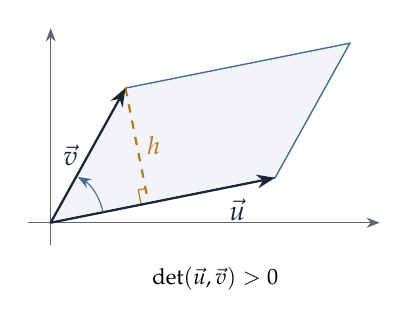
\begin{tikzpicture}[scale=0.95,>=Stealth]
  \draw[->,Gris] (-0.3,0)--(4.4,0); \draw[->,Gris] (0,-0.3)--(0,2.6);
  \fill[Fond,draw=BleuMoyen,line width=0.5pt] (0,0)--(3,0.6)--(4,2.4)--(1,1.8)--cycle;
  \draw[Ocre,dashed,line width=0.8pt] (1,1.8)--(1.3077,0.2615) node[midway,right,font=\small]{$h$};
  \draw[Ocre,line width=0.4pt] (1.2097,0.2419)--(1.1707,0.4380)--(1.2687,0.4576);
  \draw[->,thick,Ink] (0,0)--(3,0.6) node[pos=0.75,below right]{$\ve u$};
  \draw[->,thick,Ink] (0,0)--(1,1.8) node[midway,left]{$\ve v$};
  \draw[->,BleuMoyen] (0.7,0.14) arc (11:60:0.7);
  \node[font=\footnotesize\sffamily,align=center] at (2.2,-0.75) {$\det(\ve u,\ve v)>0$};
\end{tikzpicture}\hfill
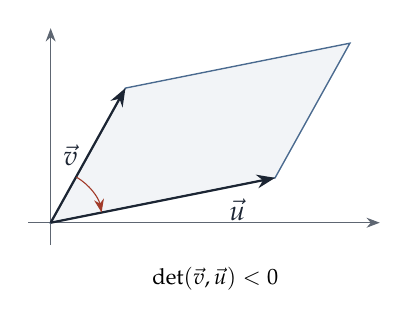
\begin{tikzpicture}[scale=0.95,>=Stealth]
  \draw[->,Gris] (-0.3,0)--(4.4,0); \draw[->,Gris] (0,-0.3)--(0,2.6);
  \fill[Fond,draw=BleuMoyen,line width=0.5pt] (0,0)--(3,0.6)--(4,2.4)--(1,1.8)--cycle;
  \draw[->,thick,Ink] (0,0)--(1,1.8) node[midway,left]{$\ve v$};
  \draw[->,thick,Ink] (0,0)--(3,0.6) node[pos=0.75,below right]{$\ve u$};
  \draw[->,Brique] (0.7*0.4903,0.7*0.8716) arc (60:11:0.7);
  \node[font=\footnotesize\sffamily] at (2.2,-0.75) {$\det(\ve v,\ve u)<0$};
\end{tikzpicture}\hfill
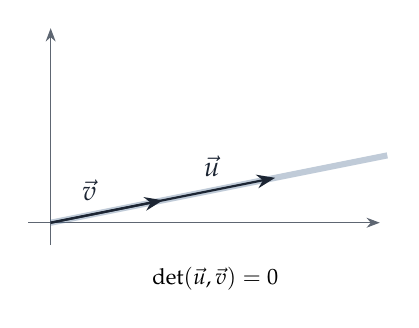
\begin{tikzpicture}[scale=0.95,>=Stealth]
  \draw[->,Gris] (-0.3,0)--(4.4,0); \draw[->,Gris] (0,-0.3)--(0,2.6);
  \draw[BleuMoyen,line width=2.2pt,opacity=0.35] (0,0)--(4.5,0.9);
  \draw[->,thick,Ink] (0,0)--(3,0.6) node[pos=0.8,above left]{$\ve u$};
  \draw[->,thick,Ink] (0,0)--(1.5,0.3) node[midway,above left]{$\ve v$};
  \node[font=\footnotesize\sffamily] at (2.2,-0.75) {$\det(\ve u,\ve v)=0$};
\end{tikzpicture}
\caption{Aire orientée. À gauche, $\ve u$ et $\ve v$ dans le sens direct ; au centre, les mêmes vecteurs dans l'ordre inverse ;
à droite, deux vecteurs colinéaires.}\label{fig:aire2}
\end{figure}

\begin{proposition}\label{prop:col}
$\det(\ve u,\ve v)=0\iff(\ve u,\ve v)$ est liée. Si $ad-bc\neq0$,
$\begin{pmatrix}a&b\\c&d\end{pmatrix}^{-1}=\dfrac1{ad-bc}\begin{pmatrix}d&-b\\-c&a\end{pmatrix}$ (on échange la diagonale, on
change le signe du reste, on divise par le déterminant).
\end{proposition}

En dimension 3, le déterminant de $(\ve u,\ve v,\ve w)$ est le \emph{produit mixte} :
\begin{equation}\label{eq:det3}
\det(\ve u,\ve v,\ve w)=\dt{a&d&g\\b&e&h\\c&f&i}=(\ve u\wedge\ve v)\cdot\ve w
=a\dt{e&h\\f&i}-b\dt{d&g\\f&i}+c\dt{d&g\\e&h}.
\end{equation}
(En pratique, règle de Sarrus : $aei+dhc+gbf-ceg-fha-ibd$.) C'est le \emph{volume orienté} du parallélépipède construit sur les trois vecteurs : aire de la base
$\|\ve u\wedge\ve v\|$ fois hauteur $h=\pm\ve w\cdot\frac{\ve u\wedge\ve v}{\|\ve u\wedge\ve v\|}$. Il est nul si et seulement
si les trois vecteurs sont coplanaires (liés).

\begin{figure}[H]
\centering
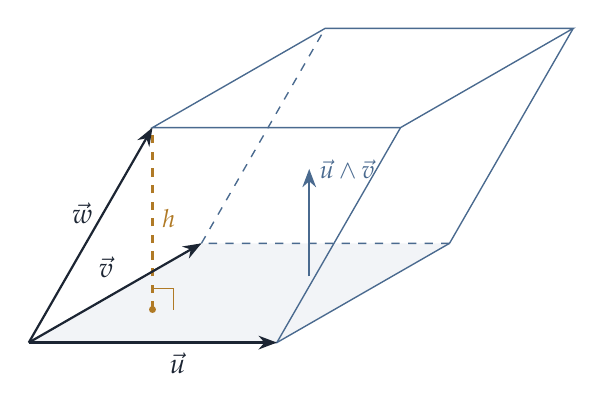
\begin{tikzpicture}[scale=1.05,>=Stealth,x={(1cm,0cm)},y={(0.62cm,0.5cm)},z={(0cm,1cm)}]
  \coordinate (O) at (0,0,0); \coordinate (U) at (3,0,0); \coordinate (V) at (0.6,2.4,0); \coordinate (W) at (1,0.8,2.2);
  \coordinate (UV) at (3.6,2.4,0); \coordinate (UW) at (4,0.8,2.2); \coordinate (VW) at (1.6,3.2,2.2); \coordinate (UVW) at (4.6,3.2,2.2);
  % base
  \fill[Fond] (O)--(U)--(UV)--(V)--cycle;
  \draw[BleuMoyen,line width=0.5pt] (O)--(U)--(UV);
  \draw[BleuMoyen,line width=0.5pt,dashed] (UV)--(V)--(O);
  % arêtes latérales et face supérieure
  \draw[BleuMoyen,line width=0.5pt] (U)--(UW) (UV)--(UVW);
  \draw[BleuMoyen,line width=0.5pt,dashed] (V)--(VW);
  \draw[BleuMoyen,line width=0.5pt] (W)--(UW)--(UVW)--(VW)--cycle;
  % hauteur
  \coordinate (Wp) at (1,0.8,0);
  \draw[Ocre,dashed,line width=0.9pt] (Wp)--(W);
  \node[Ocre,font=\small,right] at (1,0.8,1.1) {$h$};
  \draw[Ocre,line width=0.4pt] (1.25,0.8,0)--(1.25,0.8,0.25)--(1,0.8,0.25);
  \fill[Ocre] (Wp) circle (1.2pt);
  % normale
  \draw[->,thick,BleuMoyen] (2.4,1.6,0)--(2.4,1.6,1.3) node[right,font=\small]{$\ve u\wedge\ve v$};
  % vecteurs
  \draw[->,thick,Ink] (O)--(U) node[pos=0.6,below]{$\ve u$};
  \draw[->,thick,Ink] (O)--(V) node[pos=0.55,above left]{$\ve v$};
  \draw[->,thick,Ink] (O)--(W) node[pos=0.6,left]{$\ve w$};
\end{tikzpicture}\hspace{0.8cm}
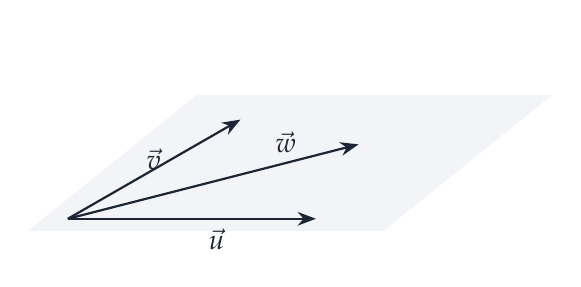
\begin{tikzpicture}[scale=1.05,>=Stealth,x={(1cm,0cm)},y={(0.62cm,0.5cm)},z={(0cm,1cm)}]
  \fill[Fond] (-0.3,-0.3,0)--(4,-0.3,0)--(4,3,0)--(-0.3,3,0)--cycle;
  \draw[->,thick,Ink] (0,0,0)--(3,0,0) node[pos=0.6,below]{$\ve u$};
  \draw[->,thick,Ink] (0,0,0)--(0.6,2.4,0) node[pos=0.6,left]{$\ve v$};
  \draw[->,thick,Ink] (0,0,0)--(2.4,1.8,0) node[pos=0.75,above]{$\ve w$};
  \node at (0,0,2.2) {};
\end{tikzpicture}
\caption{À gauche, le parallélépipède construit sur $\ve u,\ve v,\ve w$, de base grisée (aire $\|\ve u\wedge\ve v\|$) et de hauteur $h$ ; à droite, trois vecteurs coplanaires : $\ve w$ est dans le plan de $\ve u$ et $\ve v$.}\label{fig:volume}
\end{figure}

% ---------------------------------------------------------------------
\subsection{Le déterminant d'ordre $n$}


Les propriétés de l'aire et du volume orientés (§1.1) deviennent la définition en dimension $n$. On note
$C_1,\dots,C_n$ les colonnes de $A$ et l'on écrit $\det A=\det(C_1,\dots,C_n)$.

\begin{theoreme}[définition du déterminant]\label{thm:def}
Il existe une unique application $\det:\Mn{\K}\to\K$ vérifiant :
\begin{enumerate}
\item[(i)] \emph{linéarité par rapport à chaque colonne}, les autres étant fixées :
      $\det(\dots,\lambda C_j+\mu C'_j,\dots)=\lambda\det(\dots,C_j,\dots)+\mu\det(\dots,C'_j,\dots)$ ;
\item[(ii)] \emph{antisymétrie} : échanger deux colonnes change le déterminant en son opposé ;
\item[(iii)] \emph{normalisation} : $\det(I_n)=1$.
\end{enumerate}
\end{theoreme}

\emph{Lecture} (démonstration hors programme pour $n\geq4$). (i) : on peut \emph{sortir un facteur} d'une colonne et
\emph{découper} une colonne en somme --- une aire double si l'on double un côté ; (ii) : l'orientation s'inverse quand on
échange deux vecteurs ; (iii) : le cube unité a pour volume $1$. Pour $n\in\{2,3\}$, c'est le déterminant du §1.1, donc le
produit mixte ; pour $n=2$, (i), (ii), (iii) suffisent à retrouver
$\det\big(ae_1+ce_2,be_1+de_2\big)=ab\det(e_1,e_1)+ad\det(e_1,e_2)+cb\det(e_2,e_1)+cd\det(e_2,e_2)=ad-bc$, car $\det(e_1,e_1)=\det(e_2,e_2)=0$ (ii) et $\det(e_2,e_1)=-\det(e_1,e_2)=-1$.

\begin{theoreme}[développement]\label{thm:dev}
Pour tous $i,j$ (démonstration non exigible) :
\[\det A=\sum_{j=1}^n(-1)^{i+j}a_{i,j}\Delta_{i,j}\quad\text{(ligne $i$)},\qquad
\det A=\sum_{i=1}^n(-1)^{i+j}a_{i,j}\Delta_{i,j}\quad\text{(colonne $j$)},\]
où le \emph{mineur} $\Delta_{i,j}$ est le déterminant obtenu en supprimant la ligne $i$ et la colonne $j$, les signes
$(-1)^{i+j}$ formant un damier qui commence par $+$. Tout ce qui est vrai des colonnes est vrai des lignes
($\det A^T=\det A$).
\end{theoreme}

Le développement donne une définition équivalente, \emph{par récurrence} sur $n$ à partir de $\dt{a&b\\c&d}=ad-bc$ ; pour
$n=3$, on retrouve~\eqref{eq:det3}.

\begin{proposition}\label{prop:op}
\begin{enumerate}
\item Une colonne nulle, ou deux colonnes égales (ou proportionnelles) : $\det A=0$.
\item $\det(\lambda A)=\lambda^n\det A$ \quad (on sort $\lambda$ de chacune des $n$ colonnes).
\item Échange $C_i\leftrightarrow C_j$ : le signe change. Dilatation $C_i\leftarrow\lambda C_i$ : $\det$ est multiplié
      par $\lambda$. Transvection $C_i\leftarrow C_i+\lambda C_j$ ($j\neq i$) : $\det$ \emph{ne change pas}.
\end{enumerate}
\end{proposition}

\begin{proof}
Tout découle de la définition. Deux colonnes égales : les échanger ne change pas $A$ mais change le signe (ii), donc
$\det A=-\det A=0$ ; une colonne nulle s'écrit $0\cdot C$ (i). Point 2 : (i) appliquée à chacune des $n$ colonnes. Échange :
(ii) ; dilatation : (i). Transvection : par (i), $\det(\dots,C_i+\lambda C_j,\dots)=\det A+\lambda\det(\dots,C_j,\dots,C_j,\dots)=\det A$.
\end{proof}

\begin{attention}
$\det(A+B)\neq\det A+\det B$ et $\det(\lambda A)=\lambda^n\det A$, non $\lambda\det A$. Dans une transvection, la colonne
modifiée garde le coefficient $1$ ; deux opérations successives s'appliquent l'une \emph{après} l'autre (la seconde voit la
colonne déjà modifiée).
\end{attention}

\begin{theoreme}\label{thm:tri}
Le déterminant d'une matrice triangulaire est le produit de ses coefficients diagonaux.
\end{theoreme}

\begin{proof}
Par récurrence sur $n$. Si $T$ est triangulaire supérieure, sa dernière ligne vaut $(0,\dots,0,t_{n,n})$ ; en développant
selon elle, $\det T=(-1)^{n+n}t_{n,n}\Delta_{n,n}$, et $\Delta_{n,n}$ est triangulaire de diagonale
$t_{1,1},\dots,t_{n-1,n-1}$.
\end{proof}

\begin{methode}{Calculer un déterminant}\label{meth:calcul}
\begin{enumerate}
\item \emph{Regarder avant de calculer} : colonnes liées ? somme constante sur les lignes ? ligne ou colonne presque nulle ?
      structure (tridiagonale, puissances, formule en $i,j$) ? La section~\ref{sec:techniques} donne la méthode pour chaque
      structure.
\item Sinon, \emph{pivot de Gauss} : créer des zéros par transvections (en notant les échanges et les facteurs sortis)
      jusqu'à une forme triangulaire, ou jusqu'à une ligne ou colonne n'ayant qu'un coefficient non nul, selon laquelle on
      développe.
\item Avec un paramètre, \emph{garder les facteurs} : on sort tout facteur commun dès qu'il apparaît ; une forme développée
      ne se refactorise presque jamais.
\end{enumerate}
\end{methode}

\begin{exemple}[choisir la méthode]
\[D=\dt{1&2&3&4\\4&1&2&3\\3&4&1&2\\2&3&4&1}.\]
Le pivot aboutit, mais au prix de calculs où l'on se trompe facilement. Plus vite : chaque ligne a pour somme $10$. $C_1\leftarrow C_1+C_2+C_3+C_4$ puis on sort $10$ ; $L_i\leftarrow L_i-L_1$ :
\[D=10\dt{1&2&3&4\\1&1&2&3\\1&4&1&2\\1&3&4&1}=10\dt{-1&-1&-1\\2&-2&-2\\1&1&-3}=10\times(-16)=-160.\]
(Dans le $3\times3$, $C_2\leftarrow C_2-C_1$ et $C_3\leftarrow C_3-C_1$ donnent $\dt{-1&0&0\\2&-4&-4\\1&0&-4}=-16$.)
\end{exemple}

% ---------------------------------------------------------------------
\subsection{Propriétés globales}

\begin{theoreme}\label{thm:fond}
Soient $A,B\in\Mn{\K}$.
\begin{enumerate}
\item $A$ est inversible $\iff\det A\neq0\iff$ les colonnes de $A$ sont libres.
\item $\det(AB)=\det A\det B$ ; si $A$ est inversible, $\det(A^{-1})=\frac1{\det A}$ ; $\det(A^T)=\det A$.
\item Deux matrices semblables ont même déterminant : $\det(PBP^{-1})=\det P\det B\det P^{-1}=\det B$.
\end{enumerate}
\end{theoreme}

\begin{proof}
Si les colonnes sont liées, $C_i=\sum_{j\neq i}\lambda_jC_j$, la transvection $C_i\leftarrow C_i-\sum_{j\neq i}\lambda_jC_j$ rend
une colonne nulle : $\det A=0$. Si $A$ est inversible, $\det A\det A^{-1}=\det I_n=1$. (Produit et transposée : admis.)
\end{proof}

\begin{definition}
Si $E$ est de dimension $n$, de base $\mathcal B$ : $\det_{\mathcal B}(u_1,\dots,u_n)$ est le déterminant de la matrice des
coordonnées des $u_j$ dans $\mathcal B$ ; pour $f\in\LE$, $\det f=\det\Mat_{\mathcal B}(f)$, indépendant de $\mathcal B$
(matrices semblables).
\end{definition}

\begin{theoreme}\label{thm:base}
$(u_1,\dots,u_n)$ est une base de $E\iff\det_{\mathcal B}(u_1,\dots,u_n)\neq0$. $f$ est un automorphisme $\iff\det f\neq0$.
Enfin $\det(f\circ g)=\det f\det g$, $\det(\lambda f)=\lambda^n\det f$, $\det(f^{-1})=\frac1{\det f}$, $\det\Id=1$.
\end{theoreme}

Par exemple, $(1,1+X,\dots,1+X+\dots+X^n)$ est une base de $\R_n[X]$ (matrice triangulaire à diagonale de $1$), et la
dérivation $D$ de $\R_n[X]$ vérifie $\det D=0$ (matrice triangulaire à diagonale nulle) : elle n'est pas bijective.

\begin{reflexe}
Pour un endomorphisme défini géométriquement, on calcule $\det f$ dans la base où sa matrice est la plus simple (base
adaptée), jamais dans la base canonique.
\end{reflexe}

\begin{proposition}\label{prop:proj-sym}
Soit $E$ de dimension $n$. Un projecteur $p$ vérifie $\det p=1$ si $p=\Id$, $\det p=0$ sinon. Une symétrie $s$ vérifie
$\det s=(-1)^{\dim\mathrm{Ker}(s+\Id)}=(-1)^{n-\rg(s+\Id)}$.
\end{proposition}

\begin{proof}
Dans une base adaptée à $E=\mathrm{Im}\,p\oplus\mathrm{Ker}\,p$, $\Mat(p)=\mathrm{diag}(I_r,0)$. Dans une base adaptée à
$E=\mathrm{Ker}(s-\Id)\oplus\mathrm{Ker}(s+\Id)$, $\Mat(s)=\mathrm{diag}(I_r,-I_{n-r})$ ; et $\frac12(s+\Id)$ est le
projecteur sur $\mathrm{Ker}(s-\Id)$, donc $\rg(s+\Id)=r$.
\end{proof}

\begin{horsprogramme}\phantomsection\label{hp:comatrice}
\textbf{Comatrice.} La comatrice $\mathrm{com}(A)$ est la matrice des cofacteurs $(-1)^{i+j}\Delta_{i,j}$. Pour toute $A$,
$A\,\mathrm{com}(A)^T=\mathrm{com}(A)^TA=\det(A)\,I_n$, donc $A^{-1}=\frac1{\det A}\mathrm{com}(A)^T$ si $\det A\neq0$.
\emph{Pourquoi} : le coefficient $(i,i)$ de $A\,\mathrm{com}(A)^T$ est le développement de $\det A$ selon la ligne $i$ ; le
coefficient $(k,i)$, $k\neq i$, est le développement selon la ligne $i$ de la matrice où la ligne $i$ est remplacée par la
ligne $k$ : deux lignes égales, donc $0$. Utile en taille $2$ ou $3$ et pour les questions théoriques ; au-delà, le pivot
est plus rapide.
\end{horsprogramme}

\begin{exo}{td-d8}{3}{\TD{8}similitude \HP}
Soit $\C$ vu comme un $\R$-espace vectoriel. On fixe $a\in\C^*$ et l'on note $f(z)=az$, appelée similitude linéaire de
rapport $a$ dans le plan complexe.
\begin{enumerate}
\item Prouver que $f$ est bijective et déterminer $f^{-1}$.
\item À quelle condition $f$ est-elle une symétrie du plan ?
\item Calculer $\mathrm{tr}(f)$ et $\det(f)$ en fonction de $a$.
\item Si $|a|=1$, reconnaître $f$ en tant qu'application géométrique simple.
\end{enumerate}
\end{exo}
\begin{exo}{g-carre}{3}{multiplicativité ; propriété globale}
Soit $A\in\Mn{\R}$ telle que $A^2=-I_n$. Montrer que $n$ est pair. Le résultat subsiste-t-il pour une matrice complexe ?
\end{exo}
\begin{exo}{b-endo}{4}{déterminant d'un endomorphisme de matrices}
Soit $A=\begin{pmatrix}a&b\\c&d\end{pmatrix}$ et $f:\mathcal M_2(\R)\to\mathcal M_2(\R)$, $M\mapsto AM$. Montrer que
$\det f=(\det A)^2$. En déduire une condition pour que $f$ soit bijectif, et $f^{-1}$.
\end{exo}
\begin{exo}{hp-com}{3}{comatrice, coefficients entiers \HP}
\begin{enumerate}
\item Calculer la comatrice de $A=\begin{pmatrix}1&2&0\\0&1&1\\1&0&1\end{pmatrix}$ et en déduire $A^{-1}$.
\item Soit $A$ à coefficients entiers. Montrer que $A$ est inversible d'inverse à coefficients entiers si et seulement si
      $\det A=\pm1$.
\item Pour $A$ inversible, exprimer $\det(\mathrm{com}A)$ en fonction de $\det A$.
\end{enumerate}
\end{exo}

% ---------------------------------------------------------------------
\subsection{Géométrie : alignement, distances}

Le déterminant traduit directement l'alignement et la coplanarité :
$A,B,C$ alignés $\iff\det(\vv{AB},\vv{AC})=0$ ; $M\in(ABC)\iff\det(\vv{AM},\vv{AB},\vv{AC})=0$ ; aire du triangle
$=\frac12|\det(\vv{AB},\vv{AC})|$ ; volume du tétraèdre $=\frac16|\det(\vv{AB},\vv{AC},\vv{AD})|$ (base orthonormée).

\begin{proposition}\label{prop:dist-droites}
Soient $\mathcal D_1=A+\vect(\ve u)$ et $\mathcal D_2=C+\vect(\ve v)$ non parallèles. Il existe un unique couple
$(H,K)\in\mathcal D_1\times\mathcal D_2$ avec $(HK)$ perpendiculaire aux deux droites, et
\[d(\mathcal D_1,\mathcal D_2)=HK=\frac{|\det(\vv{AC},\ve u,\ve v)|}{\|\ve u\wedge\ve v\|}.\]
\end{proposition}

\begin{figure}[H]
\centering
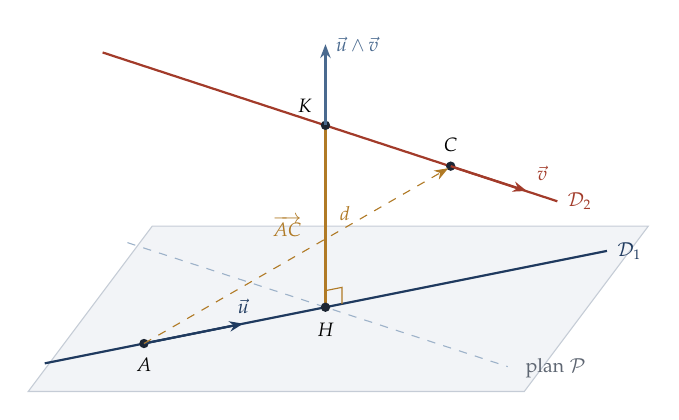
\begin{tikzpicture}[scale=1.05,>={Stealth[length=5pt]}]
\fill[Fond] (0,0)--(6,0)--(7.5,2)--(1.5,2)--cycle;
\draw[Filet] (0,0)--(6,0)--(7.5,2)--(1.5,2)--cycle;
\node[font=\scriptsize,Gris,anchor=south west] at (5.9,0.05) {plan $\mathcal P$};
% D1 dans le plan
\draw[Bleu,thick] (0.2,0.34)--(7.0,1.70) node[right,font=\scriptsize]{$\mathcal D_1$};
% projection de D2 dans le plan
\draw[BleuClair,dashed] (1.2,1.8)--(5.8,0.3);
% D2 au-dessus
\draw[Brique,thick] (0.9,4.1)--(6.4,2.3) node[right,font=\scriptsize]{$\mathcal D_2$};
% perpendiculaire commune
\draw[Ocre,thick] (3.595,1.019)--(3.595,3.219);
\draw[Ocre] (3.595,1.219)--(3.795,1.259)--(3.795,1.059);
\node[pt] at (3.595,1.019) {}; \node[font=\scriptsize,anchor=north] at (3.595,0.95) {$H$};
\node[pt] at (3.595,3.219) {}; \node[font=\scriptsize,anchor=south east] at (3.55,3.25) {$K$};
\node[font=\scriptsize,Ocre,anchor=west] at (3.65,2.15) {$d$};
% A, C et vecteurs
\node[pt] at (1.4,0.58) {}; \node[font=\scriptsize,anchor=north] at (1.4,0.52) {$A$};
\draw[->,Bleu,thick] (1.4,0.58)--(2.6,0.82) node[above,font=\scriptsize]{$\ve u$};
\node[pt] at (5.11,2.725) {}; \node[font=\scriptsize,anchor=south] at (5.11,2.78) {$C$};
\draw[->,Brique,thick] (5.11,2.725)--(6.03,2.425) node[above right,font=\scriptsize]{$\ve v$};
\draw[->,Ocre,dashed] (1.4,0.58)--(5.08,2.70) node[pos=0.55,above left,font=\scriptsize]{$\vv{AC}$};
\draw[->,BleuMoyen,thick] (3.595,3.219)--(3.595,4.2) node[right,font=\scriptsize]{$\ve u\wedge\ve v$};
\end{tikzpicture}
\caption{Deux droites non coplanaires, le plan $\mathcal P$ contenant $\mathcal D_1$ et parallèle à $\mathcal D_2$ (gris),
et la perpendiculaire commune $[HK]$ (ocre).}\label{fig:dist-droites}
\end{figure}

\emph{Lecture.} Le plan gris contient $\mathcal D_1$ et est parallèle à $\mathcal D_2$ ; la distance est la hauteur de
$\mathcal D_2$ au-dessus de ce plan. Or $|\det(\vv{AC},\ve u,\ve v)|$ est le volume du parallélépipède de base
$\|\ve u\wedge\ve v\|$ et de hauteur $d$ : on divise le volume par la base. La démonstration fait l'objet du TD~2.

\begin{exo}{td-d1}{2}{\TD{1}alignement}
Soit $A(a,a')$, $B(b,b')$ et $C(c,c')$ tels que $\dt{1&1&1\\a&b&c\\a'&b'&c'}=0$. Montrer que $A$, $B$, $C$ sont alignés dans
le plan.
\end{exo}
\begin{exo}{td-d2}{3}{\TD{2}distance de deux droites}
Soient $(AB)$ et $(CD)$ deux droites (non parallèles) de l'espace. Prouver que
\[d\big((AB),(CD)\big)=\frac{\big|\det(\vv{AB},\vv{CD},\vv{AC})\big|}{\|\vv{AB}\wedge\vv{CD}\|}.\]
\end{exo}

% ---------------------------------------------------------------------
\subsection{Techniques de calcul d'ordre $n$}\label{sec:techniques}

\subsubsection{Somme constante}

\begin{proposition}\label{prop:ab}
Le déterminant d'ordre $n$ à diagonale $a$ et autres coefficients $b$ vaut $D_n(a,b)=\big(a+(n-1)b\big)(a-b)^{n-1}$.
\end{proposition}

\begin{proof}
Chaque ligne a pour somme $s=a+(n-1)b$. $C_1\leftarrow C_1+\dots+C_n$ remplit la première colonne de $s$, que l'on sort ;
$L_i\leftarrow L_i-L_1$ ($i\geq2$) laisse une matrice triangulaire de diagonale $(1,a-b,\dots,a-b)$.
\end{proof}

\begin{exo}{td-d6}{3}{\TD{6}base et déterminant}
Soit $\mathcal B=(e_1,\dots,e_n)$ une base d'un espace vectoriel $E$ sur $\K$, et $(a,b)\in\K^2$. On pose, pour
$j\in\ient1n$, $\delta_j=ae_j+b\sum_{i\neq j}e_i$. Prouver que $\mathcal C=(\delta_1,\dots,\delta_n)$ est une base de $E$ si et
seulement si $a\neq b$ et $a+(n-1)b\neq0$.
\end{exo}

\subsubsection{Matrices définies par une formule : différences successives}

\begin{methode}{Différences successives}\label{meth:diff}
Si deux colonnes voisines se ressemblent ($a_{i,j}=\max(i,j)$, $|i-j|$, $a^{|i-j|}$\dots), on effectue
$C_k\leftarrow C_k-C_{k-1}$ (ou $C_k-aC_{k-1}$) \emph{pour $k$ allant de $n$ à $2$} --- en commençant par la fin, chaque
opération utilise une colonne intacte. On calcule le nouveau coefficient en distinguant $i<k$ et $i\geq k$ : on obtient des
blocs de $0$ et de $\pm1$, puis une matrice triangulaire ou une ligne creuse.
\end{methode}

\begin{exemple}\label{ex:max}
$A_n=\big(\max(i,j)\big)$. Après $C_k\leftarrow C_k-C_{k-1}$ ($k=n,\dots,2$), le coefficient $(i,k)$ vaut
$\max(i,k)-\max(i,k-1)=1$ si $i<k$, $0$ si $i\geq k$ ; la première colonne reste $(1,\dots,n)^T$. La dernière ligne devient
$(n,0,\dots,0)$ : en développant selon elle, $\det A_n=(-1)^{n+1}n\,\Delta_{n,1}$, avec $\Delta_{n,1}$ triangulaire à
diagonale de $1$. Donc $\det A_n=(-1)^{n+1}n$.
\end{exemple}

\begin{exo}{f-absij}{4}{différences de colonnes puis de lignes}
Calculer le déterminant $B_n$ de la matrice $\big(|i-j|\big)_{1\leq i,j\leq n}$, $n\geq2$.
\end{exo}
\begin{exo}{f-ka}{4}{différences pondérées}
Soit $a\in\R$. Calculer $\det\big(a^{|i-j|}\big)_{1\leq i,j\leq n}$.
\end{exo}

\subsubsection{Déterminants creux}

\begin{reflexe}
Une ligne (ou colonne) n'ayant qu'\emph{un} coefficient non nul : on développe selon elle, avec le signe $(-1)^{i+j}$. Deux
coefficients non nuls : on développe et les deux mineurs ont souvent la forme de départ, d'où une récurrence.
\end{reflexe}

\begin{astuce}
Permuter les lignes \emph{et} les colonnes par la \emph{même} permutation ne change pas le déterminant (les signes se
compensent ; c'est $\det(P^{-1}AP)=\det A$). On regroupe ainsi les coefficients non nuls en blocs diagonaux.
\end{astuce}

\begin{exo}{td-d4}{3}{\TD{4}déterminant en forme de X}
Pour $(a,b)\in\K^2$, calculer le déterminant de taille $2n\times2n$
\[A_{2n}=\dt{a&0&\cdots&\cdots&0&b\\0&a&&&b&0\\\vdots&&\ddots&\iddots&&\vdots\\\vdots&&\iddots&\ddots&&\vdots\\0&b&&&a&0\\b&0&\cdots&\cdots&0&a}.\]
\end{exo}
\begin{exo}{td-d9}{4}{\TD{9}déterminant en forme de Z}
Soit $n\geq3$. On considère le déterminant en forme de Z
\[D=\dt{a_1&a_2&\cdots&a_{n-1}&a_n\\0&0&\cdots&b_{n-1}&0\\\vdots&&\iddots&&\vdots\\0&b_2&\cdots&0&0\\c_1&c_2&\cdots&c_{n-1}&c_n},\]
où, pour $2\leq k\leq n-1$, la ligne $k$ ne contient que $b_{n+1-k}$, en colonne $n+1-k$. Calculer $\det(D)$ en pensant d'abord
à factoriser tout ce qui peut l'être.
\end{exo}

\subsubsection{Déterminant de Vandermonde}

\begin{theoreme}\label{thm:vdm}
$V(x_1,\dots,x_n)=\det\big(x_j^{\,i-1}\big)_{1\leq i,j\leq n}=\prod_{1\leq i<j\leq n}(x_j-x_i)$, non nul si et seulement si les
$x_i$ sont deux à deux distincts.
\end{theoreme}

\begin{methode}{Voir un déterminant comme un polynôme}\label{meth:poly}
Si une variable $x$ n'apparaît que dans une colonne, le développement selon cette colonne montre que $P(x)$ est un
polynôme, de coefficient dominant un cofacteur. On cherche ses racines évidentes (valeurs rendant deux colonnes
égales) ; si l'on en trouve autant que le degré, $P$ est le coefficient dominant fois le produit des $(x-\text{racine})$.
Démonstration du théorème : TD~5.
\end{methode}

\begin{exo}{td-d5}{4}{\TD{5}déterminant de Vandermonde}
Soit $A=\begin{pmatrix}1&1&1&1\\a&b&c&x\\a^2&b^2&c^2&x^2\\a^3&b^3&c^3&x^3\end{pmatrix}$ et $P(x)=\det(A)$.
\begin{enumerate}
\item Prouver que $P$ est un polynôme, donner son degré et ses racines.
\item En déduire la valeur de $\det(A)$ sous forme de produit de $6$ facteurs.
\item Soit $A=\big(a_j^{\,i-1}\big)_{1\leq i,j\leq n}$ ; montrer par récurrence que
      $\det(A)=\prod_{k=2}^n\prod_{p=1}^{k-1}(a_k-a_p)$.
\end{enumerate}
\end{exo}

\subsubsection{Déterminants tridiagonaux : récurrences}

\begin{methode}{Établir et résoudre une récurrence}\label{meth:rec}
Développer selon la première ligne, puis développer le second mineur selon sa première colonne : pour un tridiagonal de
diagonale $a$, de sur-diagonale $b$ et de sous-diagonale $c$ (constantes), $T_n=aT_{n-1}-bc\,T_{n-2}$. Seul le
\emph{produit} $bc$ compte. On résout avec l'équation caractéristique $r^2=ar-bc$ :
\begin{itemize}
\item deux racines distinctes $r_1,r_2$ (réelles ou complexes) : $T_n=\lambda r_1^n+\mu r_2^n$ ;
\item racine double $r$ : $T_n=(\lambda+\mu n)r^n$ ;
\item racines $e^{\pm i\theta}$ : $T_n=\lambda\cos n\theta+\mu\sin n\theta$.
\end{itemize}
On fixe $\lambda,\mu$ avec $T_1$, $T_2$ (ou $T_0=1$, valeur compatible avec la relation), et l'on vérifie $T_3$.
\end{methode}

\begin{exo}{td-d3}{3}{\TD{3}suite récurrente linéaire d'ordre 2}
Soit $A_n=\big(5\delta_{i,j}+6\delta_{i,j-1}+\delta_{i-1,j}\big)_{1\leq i,j\leq n}$.
\begin{enumerate}
\item Calculer $\det(A_4)$.
\item Soit $u_n=\det(A_n)$. Montrer que $(u_n)$ est une suite récurrente linéaire d'ordre 2 et la calculer.
\end{enumerate}
\end{exo}
\begin{exo}{td-d7}{4}{\TD{7}suite récurrente, racines complexes}
Soit $\theta\in\R$. On considère la matrice d'ordre $n$ ayant des $2\cos\theta$ sur la diagonale, des $1$ juste au-dessus et
juste au-dessous, et des $0$ ailleurs. Vérifier que $\det(A_n)=\dfrac{\sin\big((n+1)\theta\big)}{\sin\theta}$.
\end{exo}

\subsubsection{Ajouter une constante à tous les coefficients}

\begin{methode}{Fonction affine}\label{meth:affine}
Si $D(x)$ est le déterminant obtenu en ajoutant $x$ à tous les coefficients, les opérations $C_j\leftarrow C_j-C_1$
($j\geq2$) chassent $x$ de toutes les colonnes sauf la première ; par linéarité, $x\mapsto D(x)$ est \emph{affine}. On la
détermine par deux valeurs de $x$ qui rendent la matrice triangulaire.
\end{methode}

\begin{exo}{td-d10}{5}{\TD{10}polynôme de degré 1}
On note $U$ la matrice de taille $n\times n$ dont tous les coefficients valent $1$, et
\[A_n=\begin{pmatrix}\lambda_1&a&\cdots&a\\b&\lambda_2&\ddots&\vdots\\\vdots&\ddots&\ddots&a\\b&\cdots&b&\lambda_n\end{pmatrix}.\]
\begin{enumerate}
\item Soit $P(x)=\det(A_n-xU)$. Montrer que $\deg(P)\leq1$.
\item Calculer $P(a)$ et $P(b)$ et en déduire $\det(A_n)$ pour $a\neq b$.
\item À l'aide d'une dérivée, trouver $\det(A_n)$ pour $a=b$.
\end{enumerate}
\end{exo}
\begin{exo}{det-pb}{4}{fonction affine, parité, antisymétrie}
Soit $M_n(x)$ la matrice d'ordre $n\geq2$ ayant des $x$ sur la diagonale, des $1$ au-dessus et des $-1$ au-dessous.
\begin{enumerate}
\item Montrer que $\det M_n(x)=\dfrac{(x+1)^n+(x-1)^n}2$.
\item Pour quelles valeurs réelles de $x$ la matrice est-elle inversible ?
\end{enumerate}
\end{exo}

\begin{essentiel}
\small
\begin{tabular}{>{\raggedright}p{0.44\linewidth}p{0.48\linewidth}}
Structure repérée & Méthode\\\midrule
colonnes liées, rang $\leq2$ & $\det=0$ sans calcul\\
même somme sur chaque ligne & $C_1\leftarrow\sum C_j$, sortir la somme\\
$a_{i,j}$ donné par une formule ($\max$, $|i-j|$) & différences $C_k-C_{k-1}$ de $k=n$ à $2$\\
lignes à un ou deux coefficients (X, Z, N) & développer ; permuter lignes et colonnes ensemble\\
puissances successives & Vandermonde, ou polynôme en $x$\\
tridiagonal & récurrence d'ordre 2\\
constante ajoutée partout, $a$ au-dessus, $b$ au-dessous & fonction affine, cas $a=b$ par dérivée\\
relation entre matrices ($A^2=-I$, $A^T=-A$) & $\det(AB)$, $\det(\lambda A)$, $\det A^T$\\
endomorphisme géométrique & base adaptée
\end{tabular}
\end{essentiel}

\renewcommand{\ongletcouleur}{Ocre}
\section{Corrigés}\label{sec:corriges}

Chaque corrigé commence par le \emph{choix de la méthode}, signale les astuces et les pièges, et se termine par ce qu'il faut retenir. On ne le lit qu'après avoir cherché ; s'il a fallu le consulter, on refait l'exercice quelques jours plus tard, sans aide.

\subsection*{Déterminants}
\addcontentsline{toc}{subsection}{Déterminants}
\markboth{Corrigés}{}
\begin{corrige}{td-d8}
\choix{on travaille dans la base $(1,i)$ du $\R$-espace vectoriel $\C$ : on calcule $f(1)$ et $f(i)$, et tout se lit sur la
matrice.}
Posons $a=\alpha+i\beta$. $f$ est $\R$-linéaire ($f(z+\lambda z')=f(z)+\lambda f(z')$). $f(1)=\alpha+i\beta$ et
$f(i)=-\beta+i\alpha$ :
\[\Mat_{(1,i)}(f)=\begin{pmatrix}\alpha&-\beta\\\beta&\alpha\end{pmatrix}.\]
\q{1.} $f\circ g=g\circ f=\Id$ avec $g(z)=\frac za$ ($a\neq0$) : $f$ est bijective et $f^{-1}:z\mapsto a^{-1}z$.

\q{2.} $f$ est une symétrie si et seulement si $f\circ f=\Id$, soit $a^2z=z$ pour tout $z$ : $a^2=1$, $a=\pm1$. Pour $a=1$,
$f=\Id$ (symétrie triviale) ; pour $a=-1$, $f=-\Id$ est la symétrie centrale de centre $O$.

\q{3.} $\mathrm{tr}(f)=2\alpha=2\,\mathrm{Re}(a)$ et $\det(f)=\alpha^2+\beta^2=|a|^2$.

\q{4.} Si $|a|=1$, $a=e^{i\varphi}$ et la matrice est $\begin{pmatrix}\cos\varphi&-\sin\varphi\\\sin\varphi&\cos\varphi\end{pmatrix}$ :
$f$ est la rotation de centre $O$ et d'angle $\varphi=\arg a$.
\gain{le déterminant tranche la question 2 sans calcul : une réflexion (symétrie par rapport à une droite) a pour
déterminant $-1$ (proposition~\ref{prop:proj-sym}, $\dim\mathrm{Ker}(s+\Id)=1$), alors que $\det f=|a|^2>0$. Une similitude
$z\mapsto az$ n'est donc jamais une réflexion ; c'est $z\mapsto a\overline z$ ($|a|=1$) qui en donne, avec
$\det=-|a|^2$.}
\piege{$\C$ est ici un $\R$-espace vectoriel de dimension $2$ : la trace et le déterminant se calculent sur une matrice
$2\times2$ réelle, pas sur le « scalaire » $a$.}
\retenir{$\det f>0$ : $f$ conserve l'orientation (rotations, similitudes directes) ; $\det f<0$ : elle la renverse (réflexions).
Le module $|a|$ est le rapport de dilatation des longueurs, $|a|^2=\det f$ celui des aires.}
\end{corrige}
\begin{corrige}{g-carre}
\choix{on ne connaît aucun coefficient, seulement une relation : on prend le déterminant des deux membres.}
$\det(A)^2=\det(A^2)=\det(-I_n)=(-1)^n$. Comme $\det A$ est réel, $\det(A)^2\geq0$, donc $(-1)^n>0$ (il ne peut valoir $0$) : $n$
est pair. Pour une matrice complexe, $A=iI_n$ convient pour tout $n$ : le résultat tombe, car $\det(A)^2$ peut être négatif.
\retenir{relation entre matrices $\Rightarrow$ appliquer $\det$ ($\det(AB)$, $\det(\lambda A)=\lambda^n\det A$). Exemple voisin : une
matrice antisymétrique réelle d'ordre impair n'est pas inversible ($\det A=\det A^T=\det(-A)=-\det A$).}
\end{corrige}
\begin{corrige}{b-endo}
\choix{choisir l'ordre des vecteurs de base pour obtenir une matrice diagonale par blocs : $(E_{1,1},E_{2,1},E_{1,2},E_{2,2})$,
c'est-à-dire colonne par colonne, car $AM$ agit sur chaque colonne de $M$.}
$AE_{1,1}=aE_{1,1}+cE_{2,1}$, $AE_{2,1}=bE_{1,1}+dE_{2,1}$, et de même pour la seconde colonne. Dans cette base,
$\Mat(f)=\begin{pmatrix}A&0\\0&A\end{pmatrix}$ ; en développant (ou par le déterminant diagonal par blocs),
$\det f=(\det A)^2$. Donc $f$ est bijectif si et seulement si $A$ est inversible, et alors $f^{-1}(M)=A^{-1}M$.
\piege{dans l'ordre usuel $(E_{1,1},E_{1,2},E_{2,1},E_{2,2})$, la matrice n'est pas diagonale par blocs : le résultat est le
même, mais le calcul est plus long. Le choix de la base fait la moitié du travail.}
\retenir{en dimension $n$, $\det(M\mapsto AM)=(\det A)^n$ (une copie de $A$ par colonne).}
\end{corrige}
\begin{corrige}{hp-com}
\choix{on applique la formule de la comatrice (encadré du \S1.3) ; les questions 2 et 3 reposent sur
$A\,\mathrm{com}(A)^T=\det(A)I_n$.}
\q{1.} $\det A=1\cdot1-2\cdot(0-1)=3$. Les cofacteurs, ligne par ligne :
$\mathrm{com}(A)=\begin{pmatrix}1&1&-1\\-2&1&2\\2&-1&1\end{pmatrix}$, d'où
$A^{-1}=\frac13\mathrm{com}(A)^T=\frac13\begin{pmatrix}1&-2&2\\1&1&-1\\-1&2&1\end{pmatrix}$. On vérifie $AA^{-1}=I_3$.

\q{2.} Si $\det A=\pm1$, $A^{-1}=\pm\mathrm{com}(A)^T$ est entière (cofacteurs entiers). Réciproquement, $\det A$ et $\det A^{-1}$
sont des entiers de produit $1$.

\q{3.} $\det A\cdot\det\mathrm{com}(A)=\det(\det(A)I_n)=(\det A)^n$, d'où $\det\mathrm{com}(A)=(\det A)^{n-1}$.
\piege{la comatrice se \emph{transpose} avant de diviser par $\det A$ ; et chaque cofacteur porte son signe $(-1)^{i+j}$.}
\retenir{$A^{-1}=\frac1{\det A}\mathrm{com}(A)^T$ ; en taille 2 : échanger la diagonale, changer les signes du reste.}
\end{corrige}
\begin{corrige}{td-d1}
\choix{l'alignement se traduit par $\det(\vv{AB},\vv{AC})=0$. Il faut donc faire apparaître les coordonnées de $\vv{AB}$
et $\vv{AC}$, c'est-à-dire des \emph{différences} $b-a$, $c-a$ : ce sont des transvections de colonnes.}
$C_2\leftarrow C_2-C_1$ et $C_3\leftarrow C_3-C_1$ ne changent pas le déterminant :
\[\dt{1&1&1\\a&b&c\\a'&b'&c'}=\dt{1&0&0\\a&b-a&c-a\\a'&b'-a'&c'-a'}=\dt{b-a&c-a\\b'-a'&c'-a'}=\det(\vv{AB},\vv{AC}),\]
en développant selon la première ligne. Le déterminant est nul si et seulement si $\vv{AB}$ et $\vv{AC}$ sont colinéaires,
c'est-à-dire si $A$, $B$, $C$ sont alignés. On a donc l'équivalence, pas seulement l'implication demandée.
\gain{la ligne de $1$ « absorbe » le point $A$ : retrancher la première colonne transforme des points en vecteurs. En
remplaçant $C$ par un point courant $M(x,y)$, on obtient sans calcul l'équation de la droite $(AB)$ :
$\dt{1&1&1\\a&b&x\\a'&b'&y}=0$.}
\retenir{trois points $A$, $B$, $M$ du plan sont alignés si et seulement si le déterminant de la matrice dont les colonnes sont
$(1,x,y)$ pour chacun d'eux est nul. En dimension 3, même chose avec quatre points et une ligne de $1$ : coplanarité.}
\end{corrige}
\begin{corrige}{td-d2}
\choix{la distance de deux droites est la plus petite distance $MN$, $M\in(AB)$, $N\in(CD)$. On cherche le couple $(H,K)$
qui la réalise (perpendiculaire commune), puis on reconnaît dans le produit mixte un volume « base fois hauteur ».}
Notons $\ve u=\vv{AB}$, $\ve v=\vv{CD}$, $\ve n=\ve u\wedge\ve v\neq\ve0$ (droites non parallèles).

\q{1. Existence de la perpendiculaire commune.} On cherche $H=A+s\ve u$ et $K=C+r\ve v$ avec $\vv{HK}\cdot\ve u=0$ et
$\vv{HK}\cdot\ve v=0$. Comme $\vv{HK}=\vv{AC}+r\ve v-s\ve u$, c'est le système
\[s\|\ve u\|^2-r\,\ve u\cdot\ve v=\vv{AC}\cdot\ve u,\qquad s\,\ve u\cdot\ve v-r\|\ve v\|^2=\vv{AC}\cdot\ve v,\]
de déterminant $-\|\ve u\|^2\|\ve v\|^2+(\ve u\cdot\ve v)^2=-\|\ve u\wedge\ve v\|^2\neq0$ : il a une unique solution.

\q{2. $HK$ est la distance.} Pour $M\in(AB)$, $N\in(CD)$ : $\vv{MN}=\vv{HK}+(\vv{MH}+\vv{KN})$ avec
$\vv{MH}+\vv{KN}\in\vect(\ve u,\ve v)$, orthogonal à $\vv{HK}$. Par Pythagore, $MN^2=HK^2+\|\vv{MH}+\vv{KN}\|^2\geq HK^2$.

\q{3. La formule.} Par permutation circulaire, $\det(\ve u,\ve v,\vv{AC})=(\ve u\wedge\ve v)\cdot\vv{AC}$. On décompose
$\vv{AC}=\vv{AH}+\vv{HK}+\vv{KC}$ : $\vv{AH}\in\vect(\ve u)$ et $\vv{KC}\in\vect(\ve v)$ sont orthogonaux à $\ve n$, d'où
$\ve n\cdot\vv{AC}=\ve n\cdot\vv{HK}$. Comme $\vv{HK}$ est orthogonal à $\ve u$ et $\ve v$, il est colinéaire à $\ve n$ :
$|\ve n\cdot\vv{HK}|=\|\ve n\|\,HK$. Donc $HK=\frac{|\det(\ve u,\ve v,\vv{AC})|}{\|\ve u\wedge\ve v\|}$.
\gain{interprétation éclair (figure~\ref{fig:dist-droites}) : $|\det(\ve u,\ve v,\vv{AC})|$ est le volume du parallélépipède
de base $\|\ve u\wedge\ve v\|$ ; la hauteur est la distance cherchée. Retrouver la formule par « volume / base » évite de
l'apprendre.}
\piege{le point de $\vv{AC}$ est arbitraire : on peut prendre n'importe quel point de chaque droite ($\vv{AD}$, $\vv{BC}$\dots),
le résultat ne change pas. Si les droites sont parallèles, $\ve u\wedge\ve v=\ve0$ et la formule n'a pas de sens : on calcule
alors la distance d'un point de l'une à l'autre.}
\retenir{droites sécantes $\iff$ coplanaires et non parallèles $\iff\det(\vv{AC},\ve u,\ve v)=0$ avec $\ve u\wedge\ve v\neq\ve0$.
Technique réutilisable : décomposer un vecteur selon une base adaptée, puis projeter sur la normale.}
\end{corrige}
\begin{corrige}{td-d6}
\choix{« $n$ vecteurs en dimension $n$, base ? » : on calcule $\det_{\mathcal B}(\mathcal C)$ (théorème~\ref{thm:base}). La
matrice a la même somme sur chaque ligne : proposition~\ref{prop:ab}.}
La matrice de $\mathcal C$ dans $\mathcal B$ a des $a$ sur la diagonale et des $b$ ailleurs. Chaque ligne a pour somme
$a+(n-1)b$ ; $C_1\leftarrow C_1+\dots+C_n$, on sort ce facteur, puis $L_i\leftarrow L_i-L_1$ :
\[\det_{\mathcal B}(\mathcal C)=\big(a+(n-1)b\big)\dt{1&b&\cdots&b\\0&a-b&&(0)\\\vdots&&\ddots&\\0&(0)&&a-b}=\big(a+(n-1)b\big)(a-b)^{n-1}.\]
$\mathcal C$ est une base si et seulement si ce produit est non nul, c'est-à-dire $a+(n-1)b\neq0$ et $a\neq b$ (pour $n\geq2$).
\piege{pour $n=1$, $\delta_1=ae_1$ et la condition est seulement $a\neq0$ : le facteur $(a-b)^{n-1}=1$ disparaît. L'énoncé
suppose implicitement $n\geq2$.}
\gain{la matrice s'écrit $(a-b)I_n+bJ$ ($J$ : que des $1$). Cette écriture donne aussi l'inverse et les valeurs propres ; elle
revient souvent.}
\retenir{$D_n(a,b)=(a+(n-1)b)(a-b)^{n-1}$ est à connaître ; la méthode « somme constante » s'applique dès que les lignes (ou
les colonnes) ont même somme.}
\end{corrige}
\begin{corrige}{f-absij}
\choix{comme pour $\max(i,j)$ (exemple~\ref{ex:max}) : différences de colonnes, puis une seconde vague sur les lignes.}
\q{Colonnes.} Pour $k$ de $n$ à $2$, $C_k\leftarrow C_k-C_{k-1}$ : le coefficient $(i,k)$ devient $|i-k|-|i-k+1|$, soit $1$ si
$i<k$ et $-1$ si $i\geq k$. La première colonne reste $(0,1,\dots,n-1)^T$.

\q{Lignes.} Pour $i$ de $n$ à $2$, $L_i\leftarrow L_i-L_{i-1}$ : la ligne $i$ devient $(1,0,\dots,0,-2,0,\dots,0)$, le $-2$ en
colonne $i$ ; la ligne $1$ reste $(0,1,\dots,1)$.

\q{Conclure.} $C_1\leftarrow C_1+\frac12(C_2+\dots+C_n)$ annule la première colonne sauf son premier coefficient,
$\frac{n-1}2$. Matrice triangulaire de diagonale $\left(\frac{n-1}2,-2,\dots,-2\right)$ :
\[B_n=\frac{n-1}2(-2)^{n-1}=(-1)^{n-1}(n-1)2^{n-2}.\]
Contrôle : $B_2=-1$, $B_3=4$.
\gain{dans la 3\textsuperscript{e} étape, on combine les colonnes pour annuler les $1$ de la première colonne : chaque $-2$
« absorbe » un $1$ avec le coefficient $\frac12$.}
\retenir{différences de colonnes, puis de lignes : chaque vague simplifie d'un cran. Toujours dans l'ordre $k=n,n-1,\dots,2$.}
\end{corrige}
\begin{corrige}{f-ka}
\choix{au-dessus de la diagonale, la colonne $k$ vaut $a$ fois la colonne $k-1$ : on retranche $aC_{k-1}$ (et non $C_{k-1}$).}
Pour $k$ de $n$ à $2$, $C_k\leftarrow C_k-aC_{k-1}$ : pour $i<k$, $a^{k-i}-a\cdot a^{k-1-i}=0$ ; pour $i\geq k$,
$a^{i-k}-a\cdot a^{i-k+1}=a^{i-k}(1-a^2)$. Matrice triangulaire inférieure de diagonale $(1,1-a^2,\dots,1-a^2)$ :
$\det=(1-a^2)^{n-1}$.
\retenir{adapter le coefficient de la différence à la structure ; contrôle immédiat : pour $a=\pm1$, les colonnes sont égales ou
opposées, le déterminant est nul.}
\end{corrige}
\begin{corrige}{td-d4}
\choix{la première et la dernière ligne n'ont que deux coefficients non nuls, et en les supprimant on retrouve un X plus
petit : récurrence. Seconde méthode, plus rapide : regrouper les coefficients non nuls en blocs.}
\q{Méthode 1 : récurrence.} Notons $D_{2n}$ ce déterminant. En développant selon la première ligne $(a,0,\dots,0,b)$ :
$D_{2n}=a\,\Delta_{1,1}+(-1)^{1+2n}b\,\Delta_{1,2n}=a\Delta_{1,1}-b\Delta_{1,2n}$.
\begin{itemize}
\item Dans $\Delta_{1,1}$, la dernière ligne est $(0,\dots,0,a)$ ; on développe selon elle : $\Delta_{1,1}=a\,D_{2n-2}$ (le
      bloc central est le X d'ordre $2n-2$).
\item Dans $\Delta_{1,2n}$, la dernière ligne est $(b,0,\dots,0)$, en position $(2n-1,1)$, de signe $(-1)^{2n}=+1$ :
      $\Delta_{1,2n}=b\,D_{2n-2}$.
\end{itemize}
D'où $D_{2n}=(a^2-b^2)D_{2n-2}$, avec $D_2=a^2-b^2$ : $\boxed{D_{2n}=(a^2-b^2)^n}$.

\q{Méthode 2 : permutation.} On réordonne lignes \emph{et} colonnes selon $1,2n,2,2n-1,\dots,n,n+1$ ; le déterminant ne change
pas. La matrice devient diagonale par blocs, de $n$ blocs $\begin{pmatrix}a&b\\b&a\end{pmatrix}$ : $(a^2-b^2)^n$ en une ligne.
\piege{les signes du développement : le coefficient $b$ de la première ligne est en position $(1,2n)$, de signe $(-1)^{2n+1}=-1$.
Une erreur de signe donnerait $(a^2+b^2)^n$, faux dès $n=1$.}
\gain{en taille impaire $2n+1$, le coefficient central est seul sur sa ligne : on développe selon lui et l'on se ramène au cas
pair, d'où $a(a^2-b^2)^n$.}
\retenir{deux idées réutilisables : un développement qui reproduit la forme initiale donne une récurrence ; une même
permutation des lignes et des colonnes conserve le déterminant et révèle des blocs.}
\end{corrige}
\begin{corrige}{td-d9}
\choix{les lignes $2$ à $n-1$ n'ont qu'un coefficient : on les « sort », puis on s'en sert comme pivots pour nettoyer les lignes
$1$ et $n$.}
\q{Factoriser.} On sort $b_{n+1-k}$ de chaque ligne $k$ ($2\leq k\leq n-1$) : facteur $b_2b_3\cdots b_{n-1}$ ; la ligne $k$ devient le
vecteur ligne $e_{n+1-k}$ (un $1$ en colonne $n+1-k$).

\q{Nettoyer.} Pour chaque colonne $j\in\ient2{n-1}$, on retranche à la ligne $1$ (resp. $n$) $a_j$ (resp. $c_j$) fois la ligne
ayant un $1$ en colonne $j$ (transvections) : les lignes $1$ et $n$ deviennent $(a_1,0,\dots,0,a_n)$ et $(c_1,0,\dots,0,c_n)$.

\q{Remettre dans l'ordre.} Les lignes $2$ à $n-1$ forment une « anti-identité » sur les colonnes $2$ à $n-1$. Inverser l'ordre
de ces $n-2$ lignes demande $\left\lfloor\frac{n-2}2\right\rfloor$ échanges. On obtient alors une identité au centre ; en
développant selon les lignes $2,\dots,n-1$ (un seul $1$, en position diagonale, signe $+$), il reste
$\dt{a_1&a_n\\c_1&c_n}$. Donc
\[\det D=(-1)^{\lfloor\frac{n-2}2\rfloor}\,b_2b_3\cdots b_{n-1}\,(a_1c_n-a_nc_1).\]
Contrôle : $n=3$, $D=\dt{a_1&a_2&a_3\\0&b_2&0\\c_1&c_2&c_3}=b_2(a_1c_3-a_3c_1)$, en développant selon la ligne 2.
\gain{le nombre d'échanges pour inverser $m$ objets est $\lfloor m/2\rfloor$ (on échange le premier et le dernier, etc.) ; la
parité de $\lfloor m/2\rfloor$ est celle de $\frac{m(m-1)}2$.}
\piege{oublier le signe de l'anti-diagonale. Le déterminant « en N » (les $b_j$ sur la diagonale au lieu de l'anti-diagonale)
n'a pas ce signe : $b_2\cdots b_{n-1}(a_1c_n-a_nc_1)$.}
\retenir{face à une ligne n'ayant qu'un coefficient : la sortir comme facteur, puis l'utiliser comme pivot. Toujours tester la
formule finale sur $n=3$ ou $4$.}
\end{corrige}
\begin{corrige}{td-d5}
\choix{$x$ n'apparaît que dans la dernière colonne : méthode~\ref{meth:poly}. On ne développe surtout pas « à la main » : on
utilise la structure (degré, coefficient dominant, racines).}
\q{1.} En développant selon la dernière colonne $(1,x,x^2,x^3)^T$,
$P(x)=\gamma_0+\gamma_1x+\gamma_2x^2+\gamma_3x^3$, où les $\gamma_k$ sont des cofacteurs indépendants de $x$ : $P$ est un
polynôme de degré au plus $3$. Son coefficient de $x^3$ est le cofacteur $(-1)^{4+4}\Delta_{4,4}$,
\[\gamma_3=\dt{1&1&1\\a&b&c\\a^2&b^2&c^2}=(b-a)(c-a)(c-b)\]
(Vandermonde d'ordre 3 : $C_2\leftarrow C_2-C_1$, $C_3\leftarrow C_3-C_1$, puis on sort $b-a$ et $c-a$). Enfin $P(a)=P(b)=P(c)=0$
(deux colonnes égales).
\begin{itemize}
\item Si $a,b,c$ sont distincts, $\gamma_3\neq0$ : $P$ est de degré $3$ et ses racines sont exactement $a$, $b$, $c$.
\item Sinon, $A$ a deux colonnes égales pour tout $x$ : $P=0$.
\end{itemize}
\q{2.} Un polynôme de degré $3$ de coefficient dominant $\gamma_3$ et de racines $a,b,c$ vaut $\gamma_3(x-a)(x-b)(x-c)$ :
\[\det A=(b-a)(c-a)(c-b)(x-a)(x-b)(x-c),\]
formule vraie aussi lorsque $a,b,c$ ne sont pas distincts (les deux membres sont nuls).

\q{3.} Notons $V_n(a_1,\dots,a_n)$ ce déterminant. La propriété est vraie pour $n=2$ : $V_2=a_2-a_1$. Supposons-la vraie au rang
$n-1$. Remplaçons $a_n$ par $x$ : comme en 1, $Q(x)=V_n(a_1,\dots,a_{n-1},x)$ est un polynôme de degré au plus $n-1$, de
coefficient de $x^{n-1}$ égal au cofacteur $V_{n-1}(a_1,\dots,a_{n-1})$, et s'annule en $a_1,\dots,a_{n-1}$. Si les $a_p$
($p<n$) sont distincts, $Q(x)=V_{n-1}(a_1,\dots,a_{n-1})\prod_{p=1}^{n-1}(x-a_p)$ ; sinon les deux membres sont nuls. En
$x=a_n$ et par hypothèse de récurrence :
\[V_n=\prod_{k=2}^{n-1}\prod_{p=1}^{k-1}(a_k-a_p)\times\prod_{p=1}^{n-1}(a_n-a_p)=\prod_{k=2}^n\prod_{p=1}^{k-1}(a_k-a_p).\]
\gain{le coefficient dominant se lit sans calcul : c'est le mineur qui reste quand on barre la ligne et la colonne de
$x^{n-1}$. Et les racines évidentes viennent de « deux colonnes égales ».}
\piege{oublier le cas où les $a_p$ ne sont pas distincts (le degré chute) ; il se règle en une phrase, mais il faut l'écrire.}
\retenir{la méthode du polynôme s'applique dès qu'une variable n'occupe qu'une ligne ou une colonne. $V\neq0\iff$ les points
sont distincts : c'est l'outil de l'interpolation de Lagrange et de la liberté des familles $(x\mapsto e^{\alpha_ix})$.}
\end{corrige}
\begin{corrige}{td-d3}
\choix{commencer par \emph{dessiner} la matrice : les symboles de Kronecker cachent un tridiagonal. Puis méthode~\ref{meth:rec}.}
$\delta_{i,j-1}=1$ si et seulement si $j=i+1$ : des $6$ juste au-dessus de la diagonale ; $\delta_{i-1,j}=1$ si et seulement si
$i=j+1$ : des $1$ juste au-dessous ; des $5$ sur la diagonale.
\[A_4=\begin{pmatrix}5&6&0&0\\1&5&6&0\\0&1&5&6\\0&0&1&5\end{pmatrix}.\]
\q{Récurrence.} On développe $u_n$ selon la première ligne $(5,6,0,\dots,0)$ :
$u_n=5u_{n-1}-6\Delta_{1,2}$. Le mineur $\Delta_{1,2}$ a pour première colonne $(1,0,\dots,0)^T$ ; en le développant selon
elle, $\Delta_{1,2}=1\cdot u_{n-2}$. Donc
\[u_n=5u_{n-1}-6u_{n-2}\quad(n\geq3),\qquad u_1=5,\ u_2=25-6=19.\]
\q{1.} $u_3=5\cdot19-6\cdot5=65$, puis $\det(A_4)=u_4=5\cdot65-6\cdot19=211$.

\q{2.} L'équation caractéristique $r^2-5r+6=0$ a pour racines $2$ et $3$ : $u_n=\alpha2^n+\beta3^n$. Avec
$2\alpha+3\beta=5$ et $4\alpha+9\beta=19$ : $\beta=3$, $\alpha=-2$, d'où
\[u_n=3^{n+1}-2^{n+1}.\]
Contrôle : $u_4=243-32=211$.
\gain{on peut poser $u_0=1$ (valeur qui rend la relation vraie pour $n=2$ : $19=5\cdot5-6u_0$) : les conditions $u_0=1$, $u_1=5$
donnent les constantes plus vite. Et seul le produit $6\times1$ des coefficients hors diagonale compte : échanger $6$ et $1$ ne
change rien.}
\piege{oublier le signe $(-1)^{1+2}=-1$ du coefficient $6$, ce qui donne $u_n=5u_{n-1}+6u_{n-2}$ ; le contrôle sur $u_3$ (calculé
par Sarrus) détecte l'erreur.}
\retenir{tridiagonal (diagonale $a$, voisins $b$ et $c$) $\Rightarrow T_n=aT_{n-1}-bc\,T_{n-2}$ ; toujours vérifier la formule
finale sur un petit $n$.}
\end{corrige}
\begin{corrige}{td-d7}
\choix{tridiagonal : récurrence (méthode~\ref{meth:rec}). Comme le résultat est donné, la vérification par récurrence avec une
formule de trigonométrie est plus courte que la résolution.}
Notons $D_n=\det(A_n)$. Le développement donne $D_n=2\cos\theta\,D_{n-1}-D_{n-2}$ ($bc=1$), avec $D_1=2\cos\theta$ et
$D_2=4\cos^2\theta-1$. On suppose $\theta\notin\pi\Z$.
\begin{itemize}
\item $\frac{\sin2\theta}{\sin\theta}=2\cos\theta=D_1$ et $\frac{\sin3\theta}{\sin\theta}=4\cos^2\theta-1=D_2$, car
      $\sin3\theta=3\sin\theta-4\sin^3\theta=\sin\theta(4\cos^2\theta-1)$.
\item Si la formule est vraie aux rangs $n-1$ et $n-2$, la formule
      $\sin\big((n+1)\theta\big)+\sin\big((n-1)\theta\big)=2\sin(n\theta)\cos\theta$ donne
      $2\cos\theta D_{n-1}-D_{n-2}=\frac{\sin((n+1)\theta)}{\sin\theta}$ : elle est vraie au rang $n$.
\end{itemize}
Si $\theta\in\pi\Z$, $\cos\theta=\varepsilon=\pm1$ : racine double $\varepsilon$, et $D_n=(n+1)\varepsilon^n$, qui est la
limite de $\frac{\sin((n+1)\theta)}{\sin\theta}$.
\gain{pour \emph{trouver} la formule sans la connaître : $r^2-2\cos\theta\,r+1=0$ a pour racines $e^{\pm i\theta}$, donc
$D_n=\lambda\cos n\theta+\mu\sin n\theta$ ; avec $D_0=1$ et $D_1=2\cos\theta$, on obtient $\lambda=1$,
$\mu=\frac{\cos\theta}{\sin\theta}$, et $D_n=\frac{\sin\theta\cos n\theta+\cos\theta\sin n\theta}{\sin\theta}$.}
\piege{la formule n'a pas de sens pour $\theta\in\pi\Z$ : il faut traiter ce cas à part (racine double).}
\retenir{prolongement classique : $D_n=0\iff\theta=\frac{k\pi}{n+1}$ ($1\leq k\leq n$). Le déterminant d'ordre $n$ à diagonale $x$
et voisins $1$ est un polynôme unitaire de degré $n$ ; il a ces $n$ racines distinctes $2\cos\frac{k\pi}{n+1}$, donc n'en a pas
d'autre.}
\end{corrige}
\begin{corrige}{td-d10}
\choix{retrancher $x$ partout transforme les coefficients constants $a$ et $b$ en $a-x$ et $b-x$ : pour $x=a$ ou $x=b$, la
matrice devient triangulaire. Il suffit donc de savoir que $P$ est affine (méthode~\ref{meth:affine}).}
Notons $Q(x)=\prod_{i=1}^n(\lambda_i-x)$.

\q{1.} Les colonnes de $A_n-xU$ sont $C_j-xU_1$, où $U_1=(1,\dots,1)^T$. Les transvections $C_j\leftarrow C_j-C_1$ ($j\geq2$)
donnent des colonnes $C_j-C_1$ indépendantes de $x$ ; seule la première, $C_1-xU_1$, dépend de $x$. Par linéarité selon la
première colonne :
\[P(x)=\det(C_1,C_2-C_1,\dots)-x\det(U_1,C_2-C_1,\dots)=\beta-\alpha x :\quad\deg P\leq1.\]
\q{2.} $A_n-aU$ a des $0$ au-dessus de la diagonale : triangulaire inférieure, $P(a)=\prod(\lambda_i-a)=Q(a)$. De même
$P(b)=Q(b)$. Comme $\det A_n=P(0)$ et que $P$ est affine, on écrit la droite passant par $(a,Q(a))$ et $(b,Q(b))$ :
\[\det A_n=P(0)=\frac{b\,Q(a)-a\,Q(b)}{b-a}\qquad(a\neq b).\]
(Vérification : en $x=a$, la droite $x\mapsto\frac{(b-x)Q(a)-(a-x)Q(b)}{b-a}$ vaut bien $Q(a)$.)

\q{3.} Pour $a$ fixé, $b\mapsto\det A_n$ est polynomiale, donc continue : on fait tendre $b$ vers $a$. Avec
$\varphi(u)=u\,Q(a)-a\,Q(u)$, on a $\varphi(a)=0$ et $\det A_n=\frac{\varphi(b)-\varphi(a)}{b-a}\to\varphi'(a)$. D'où, pour $a=b$,
\[\det A_n=Q(a)-aQ'(a)=\prod_{i=1}^n(\lambda_i-a)+a\sum_{j=1}^n\prod_{i\neq j}(\lambda_i-a).\]
Contrôle : tous les $\lambda_i$ égaux à $\lambda$ : $(\lambda-a)^n+na(\lambda-a)^{n-1}=(\lambda+(n-1)a)(\lambda-a)^{n-1}$, c'est la
proposition~\ref{prop:ab}.
\gain{reconnaître un \emph{taux d'accroissement} : une expression $\frac{\varphi(b)-\varphi(a)}{b-a}$ avec $\varphi(a)=0$ tend vers
$\varphi'(a)$. C'est le sens de « à l'aide d'une dérivée ».}
\piege{en 3, on ne peut pas faire $b=a$ dans la formule de la question 2 (division par $0$) ; il faut justifier le passage à la
limite par la continuité du déterminant.}
\retenir{trois techniques : (i) $x$ ajouté partout $\Rightarrow$ affine ; (ii) choisir les valeurs de $x$ qui rendent la matrice
triangulaire ; (iii) prolonger une formule par continuité, la limite étant une dérivée.}
\end{corrige}
\begin{corrige}{det-pb}
\choix{coefficients constants au-dessus et au-dessous : c'est la situation du TD~10, que l'on applique avec $\lambda_i=x$,
$a=1$, $b=-1$.}
\q{1.} Avec $D(c)$ le déterminant obtenu en ajoutant $c$ partout (affine) : $D(-1)=(x-1)^n$ (triangulaire inférieure),
$D(1)=(x+1)^n$ (triangulaire supérieure), et pour une fonction affine $D(0)=\frac{D(1)+D(-1)}2$.

\q{2.} $n$ pair : somme de deux puissances paires qui ne s'annulent pas ensemble, $\det>0$ : toujours inversible. $n$ impair :
$(x+1)^n=(1-x)^n\iff x+1=1-x\iff x=0$ (injectivité de $u\mapsto u^n$) : inversible si et seulement si $x\neq0$.
\retenir{pour $x=0$, $M_n(0)$ est antisymétrique : on retrouve qu'en ordre impair son déterminant est nul.}
\end{corrige}


% =====================================================================
%                     INDEX DE CONSULTATION
% =====================================================================
\clearpage
\ongletsfalse
\section*{Index de consultation}\label{sec:index}
\addcontentsline{toc}{section}{Index de consultation}
\markboth{Index de consultation}{}

\subsection*{Correspondance avec le cours, les TD et le devoir}\phantomsection\label{sec:corresp}
{\footnotesize

\paragraph{Cours --- Déterminants}
\noindent Définition : linéarité, antisymétrie, $\det I_n=1$\dotfill th.~\ref{thm:def}, p.~\pageref{thm:def}\par
\noindent Développement, mineurs $\Delta_{i,j}$, définition par récurrence\dotfill th.~\ref{thm:dev}, p.~\pageref{thm:dev}\par
\noindent Aire orientée, $\|\ve u\|\|\ve v\|\sin(\ve u,\ve v)$, inverse $2\times2$\dotfill p.~\pageref{prop:col}\par
\noindent Volume, produit mixte\dotfill p.~\pageref{eq:det3}\par
\noindent Matrice triangulaire (preuve par récurrence), pivot, exemple $4\times4$\dotfill th.~\ref{thm:tri}, p.~\pageref{thm:tri}\par
\noindent Comatrice \HP\dotfill p.~\pageref{hp:comatrice}, ex.~\ref{e:hp-com}\par
\noindent $\det(AB)$, $\det(\lambda A)$, $\det A^{-1}$, $\det A^T$, bases, $\det f$, matrices semblables\dotfill p.~\pageref{thm:fond}\par
\noindent Projecteurs et symétries\dotfill prop.~\ref{prop:proj-sym}\par
\noindent Matrices $\max(i,j)$ et $|i-j|$\dotfill ex.~\ref{ex:max}, ex.~\ref{e:f-absij}\par
\paragraph{TD --- Déterminants}
\noindent 1.~Alignement \dotfill ex.~\ref{e:td-d1}\quad 2.~Distance de deux droites\dotfill ex.~\ref{e:td-d2}\par
\noindent 3.~Récurrence d'ordre 2 \dotfill ex.~\ref{e:td-d3}\quad 4.~Déterminant en X\dotfill ex.~\ref{e:td-d4}\par
\noindent 5.~Vandermonde \dotfill ex.~\ref{e:td-d5}\quad 6.~Base et déterminant\dotfill ex.~\ref{e:td-d6}\par
\noindent 7.~Récurrence, $2\cos\theta$ \dotfill ex.~\ref{e:td-d7}\quad 8.~Similitude \HP\dotfill ex.~\ref{e:td-d8}\par
\noindent 9.~Déterminant en Z \dotfill ex.~\ref{e:td-d9}\quad 10.~Polynôme de degré 1\dotfill ex.~\ref{e:td-d10}\par
}

\subsection*{Méthodes}
{\footnotesize\begin{multicols}{2}\listemethodes\end{multicols}}

\end{document}
